\documentclass{beamer}

\usepackage{hyperref}
\usepackage{graphicx}
\graphicspath{ {images/} }
\usepackage{tabularx}

\usetheme{Madrid}
\usecolortheme{default}
\setbeamertemplate{navigation symbols}{}

\begin{document}

\title{Gamification of Clinical Practice Guidelines}
\author{Ben-Richard Ebbesvik}
\institute{Western Norway University of Applied Sciences \newline University of Bergen}
\date{June 2019}
\subject{Master thesis}
\frame{\titlepage}


\begin{frame}{Introduction}
\textbf{Clinical Practice Guidelines} are documents that contain recommendations to assist clinicians providing optimized health care, based on latest evidence. 

Some advantages:
\begin{itemize}
	\item Clinicians don't have to search through and review an overwhelming amount of research articles to keep up to date with the latest best evidence.
	\item Improved quality of health care (benefits and harm).
	\item Reduce practice variability.
	\item Reduce cost of health care.
\end{itemize}	
%\begin{block}{Definition}	
%	 "Clinical Practice Guidelines are statements that include recommendations intended to optimize patient care that are informed by a systematic review of evidence and an assessment of the cost, benefits and harms of alternative care options." (The Institute of Medicine 2011)
%\end{block}
\end{frame}

\begin{frame}{Introduction}
Despite the advantages, Clinical Practice Guidelines have had a limited effect on changing clinicians practice methods.
\begin{block}{Cabana et al 1999}
\begin{itemize}
	\item Lack of awareness.
	\item Lack of familiarity.
	\item  Lack of self-efficacy.
	\item Inertia of previous practice.
	\item Not easy to use, inconvenient, cumbersome.

Example: Guidelines for the Diagnosis and Management of Asthma consists of 440 pages.
\end{itemize}
%Our contribution: a game.
\end{block}
\end{frame}

\begin{frame}{Possible asthma in paediatrics - Norway}
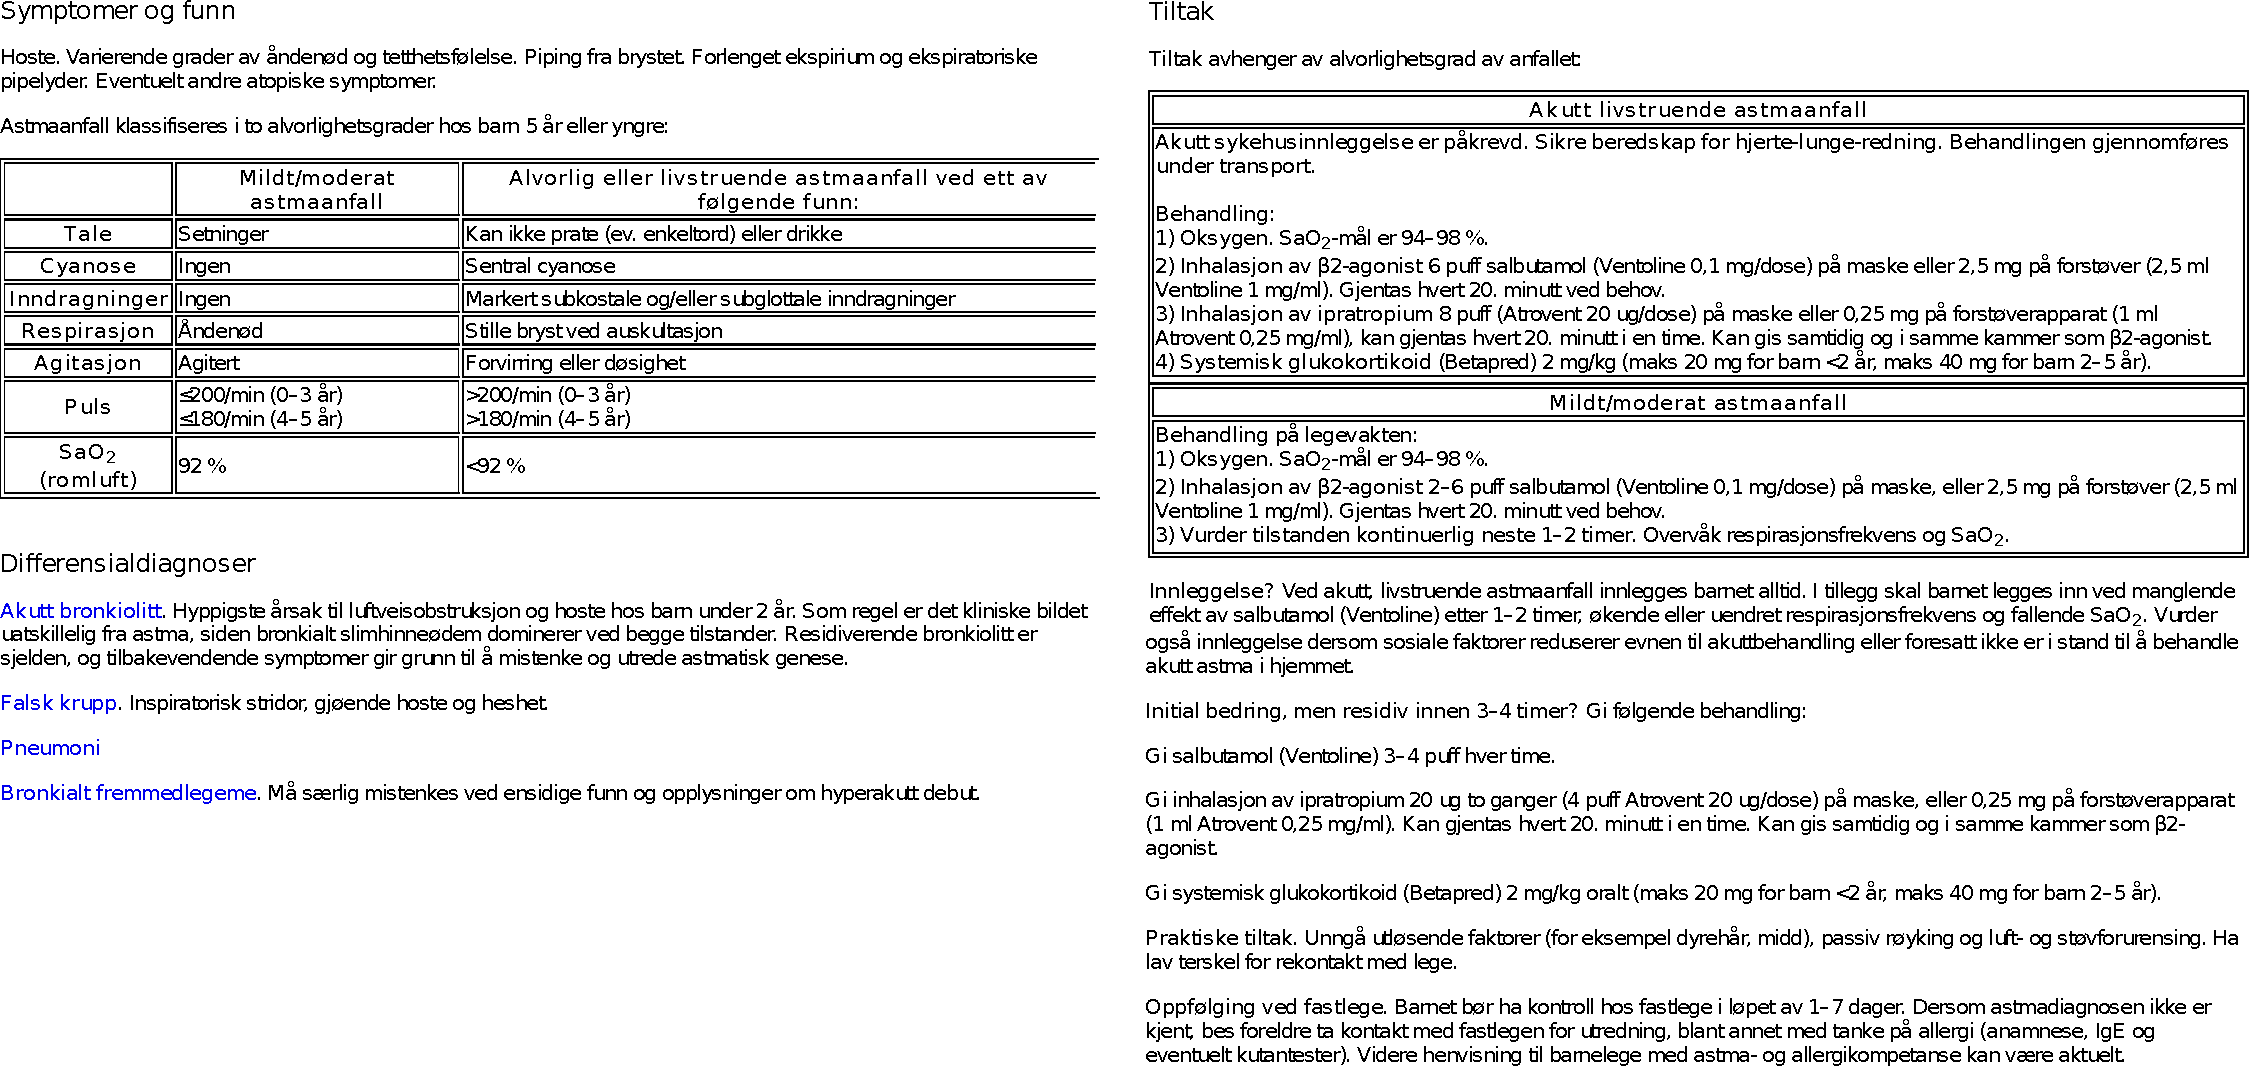
\includegraphics[scale=0.32]{NorwayCPG}
\end{frame}


\begin{frame}{Research questions}
\begin{itemize}
	\item \textbf{RQ1:} Based on clinical guidelines, how can we define and represent a generic data structure that can be used to implement applications such as online guidelines or training games for such guidelines, and where applications can adapt to the level of their users?
	\item \textbf{RQ2:} Can the generic data structure in RQ1 be used to generate a specific data model for another domain such as paediatric asthma?
	\item \textbf{RQ3:} How can we use the data model in RQ2 to implement a game for guideline training that can adapt to the level and progression  of users?
	\item \textbf{RQ4:} Is the guideline metamodel at an abstraction level such that it can be used for other guidelines? 
\end{itemize}
\end{frame}

\begin{frame}{Research method}
\begin{block}{Design science (Hevner et al 2004)}
	\begin{itemize}
		\item \textbf{Problem:} CPGs have proven to have a great potential, but are not used enough.
		\item \textbf{Design an artefact} that will contribute to more use of clinical guidelines.
		\item \textbf{Iterations:} Evaluation of the artefact will give us more knowledge around the domain and challenges. Improve and adjust the artefact accordingly. The research will appear from the design.
		\item \textbf{Contribution:} Scientific contribution to health informatics. The artefact will provide value to the medical community.
	\end{itemize}
\end{block}
\end{frame}

\begin{frame}{Gamification of Clinical Practice Guidelines}
\begin{block}{The artefact}
	\begin{itemize}
		\item A mobile game in a quiz format for learning the content of CPGs.
		\item Multiple-choice and multiple-try with feedback.
		\item Adaptive to the knowledge and progression of the individual learner.
		\item Intended for medical students and clinicians.
	\end{itemize}
\end{block}
\end{frame}

\begin{frame}{Related work: MDE gamification of CPGs}
\begin{itemize}
	\item Ontology-Based Generation of Medical, Multi-term MCQs (Leo, Kurdi, Matentzoglu et al 2019).
	\item Models and mechanisms for implementing playful scenarios (Aouadi, Pernelle, Amar, Carro, Talbot 2016).
\end{itemize}
\end{frame}

\begin{frame}{Related work: modelling}
\begin{itemize}
	\item Dynamic content manager - A new conceptual model for e-learning (Kristensen, Lamo, Hinna, Hole 2009).
	\item A	diagrammatic formalisation of mof-based modelling languages (Rutle, Rossini, Lamo, Wolter, 2009).
	\item Coordination of multiple metamodels, with application to healthcare systems (Rabbi, Lamo, MacCaull, 2014).
	\item The effects of different forms of	feedback on fuzzy and verbatim memory of science principles (Clariana, Koul 2006).
\end{itemize}
\end{frame}

\begin{frame}{Architecture}
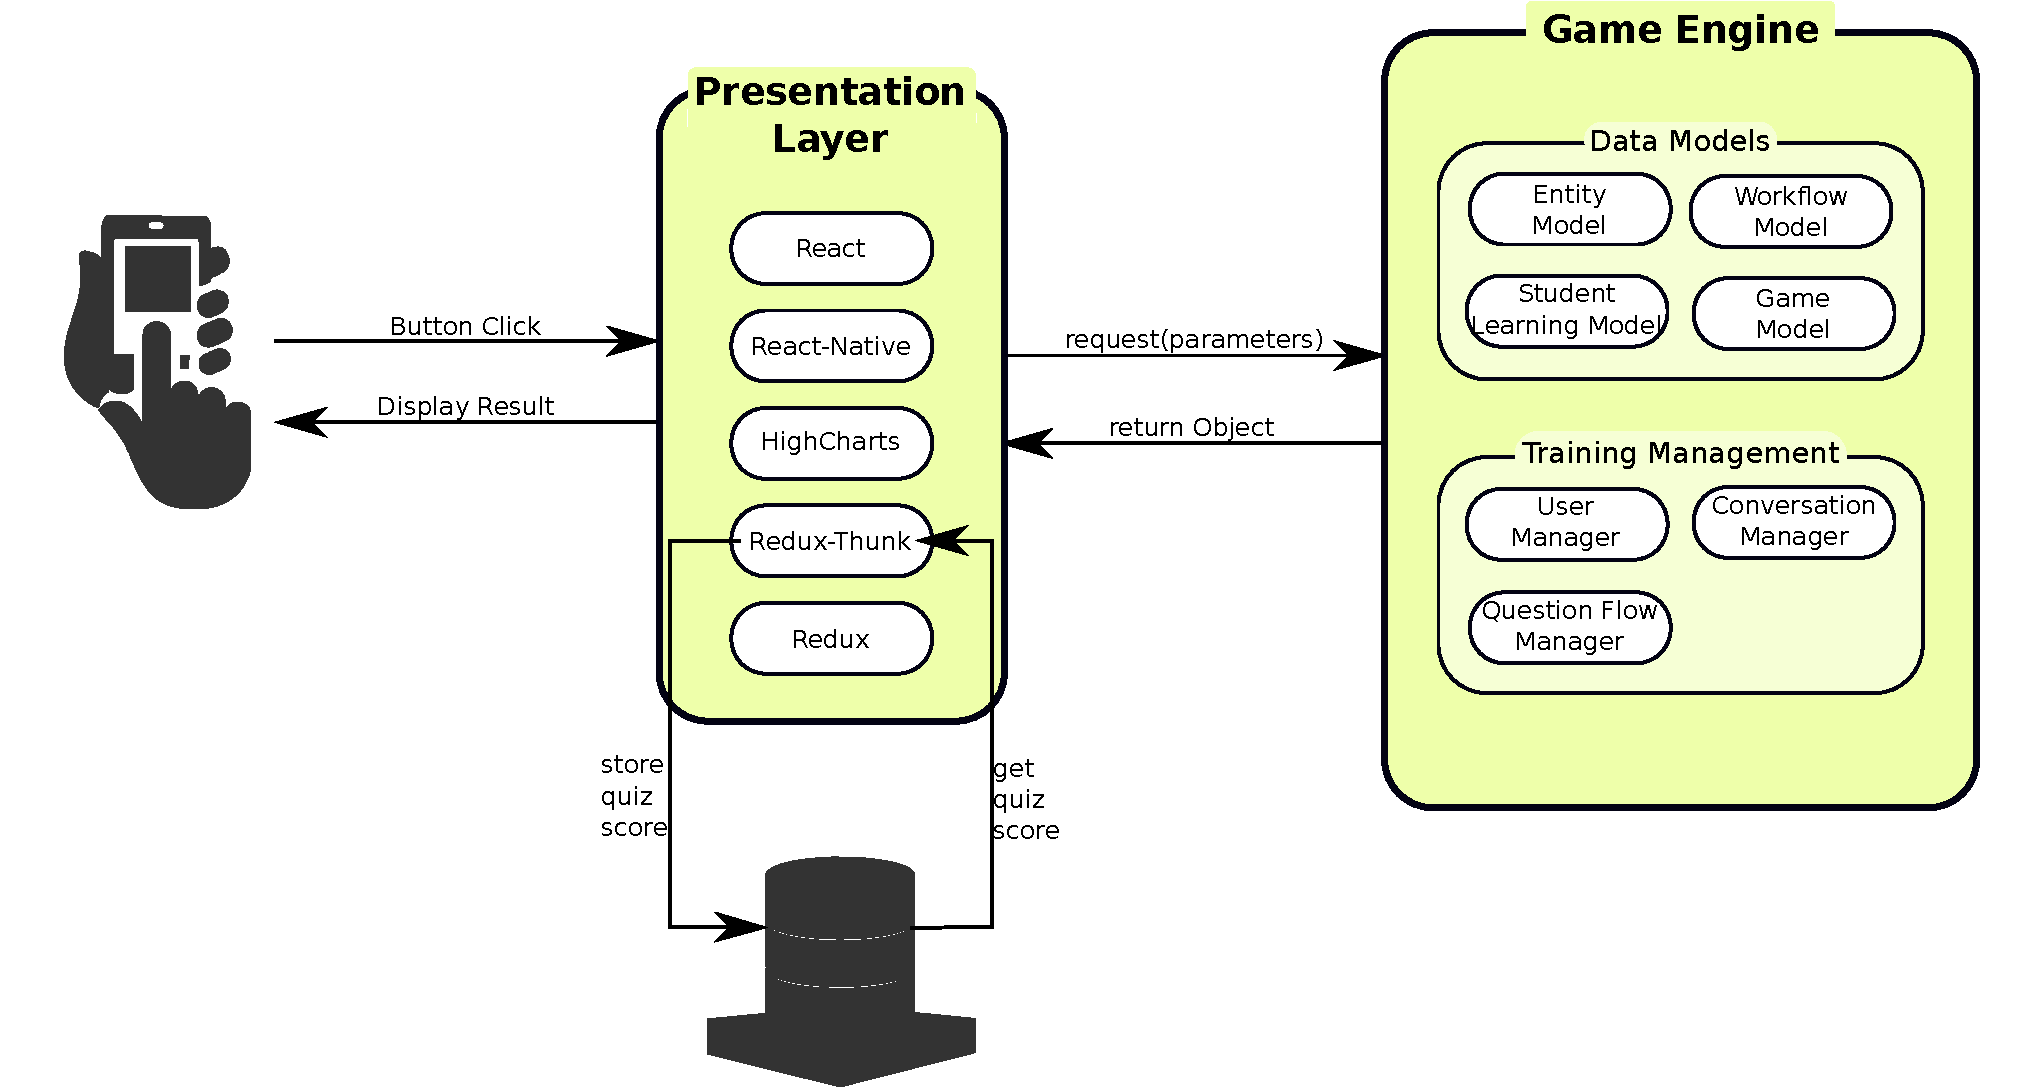
\includegraphics[scale=0.35]{Architecture}
\end{frame}

\begin{frame}{Possible asthma in paediatrics - Kenya}
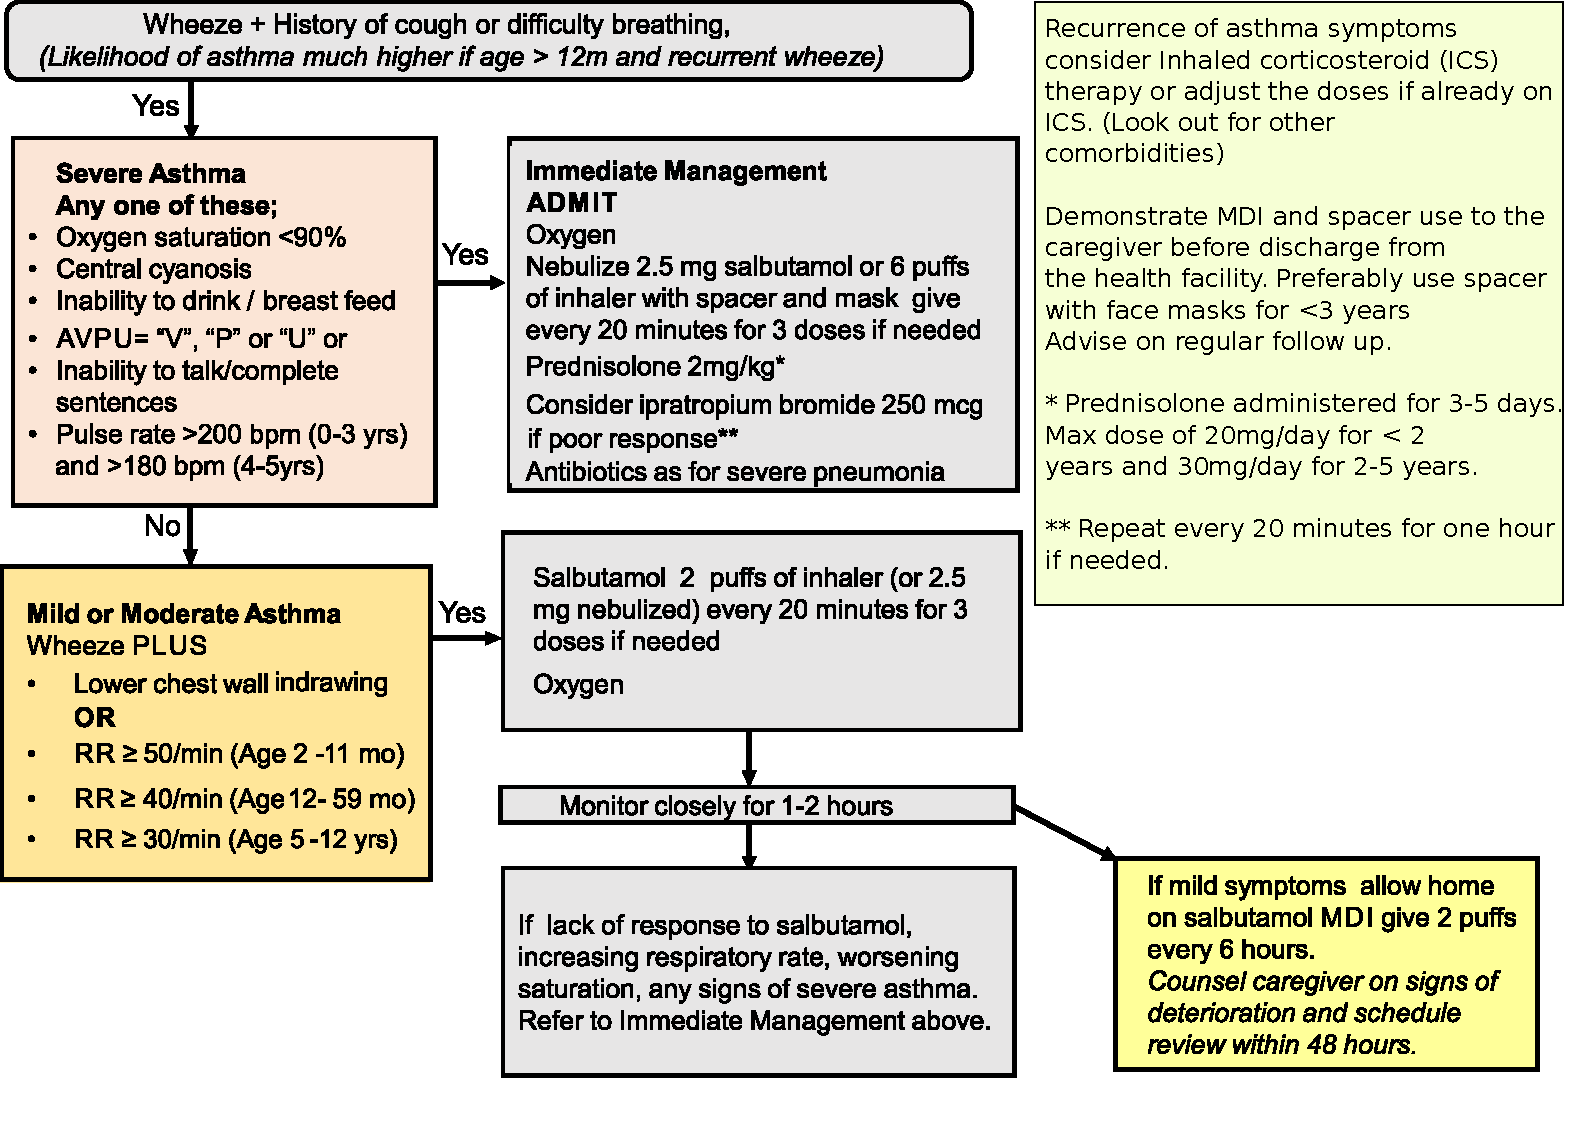
\includegraphics[scale=0.45]{KenyaCPG}
\end{frame}



\begin{frame}{Workflow graph}
The workflow graph is a model of the different steps through a clinical encounter.
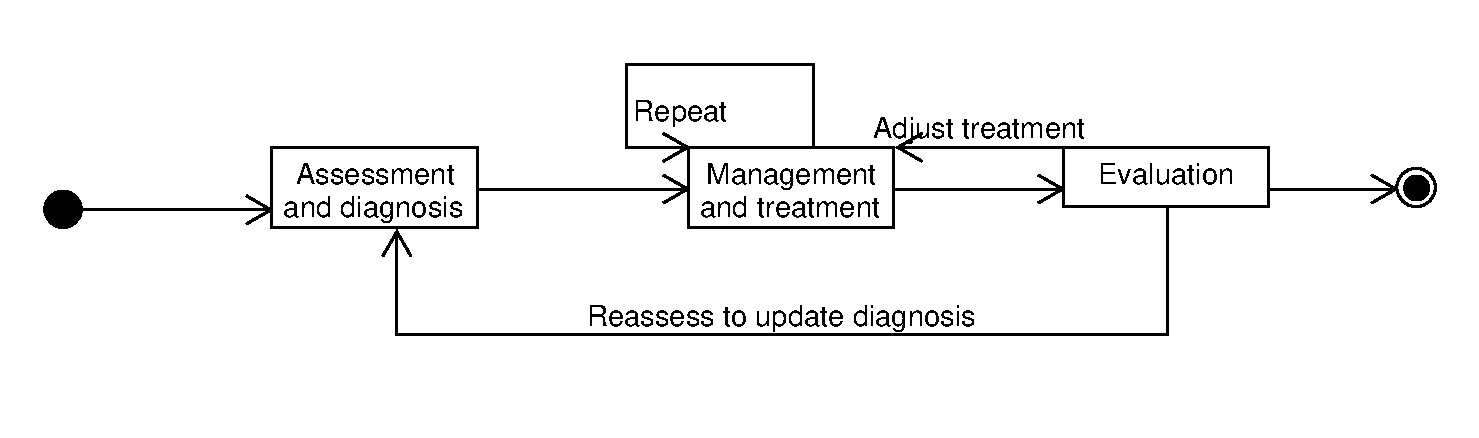
\includegraphics[scale=0.44]{WorkflowGraph}
\end{frame}

\begin{frame}{Excerpt of the entity graph}
The entity graph is a model of the patient profile at a specific point in the clinical encounter.
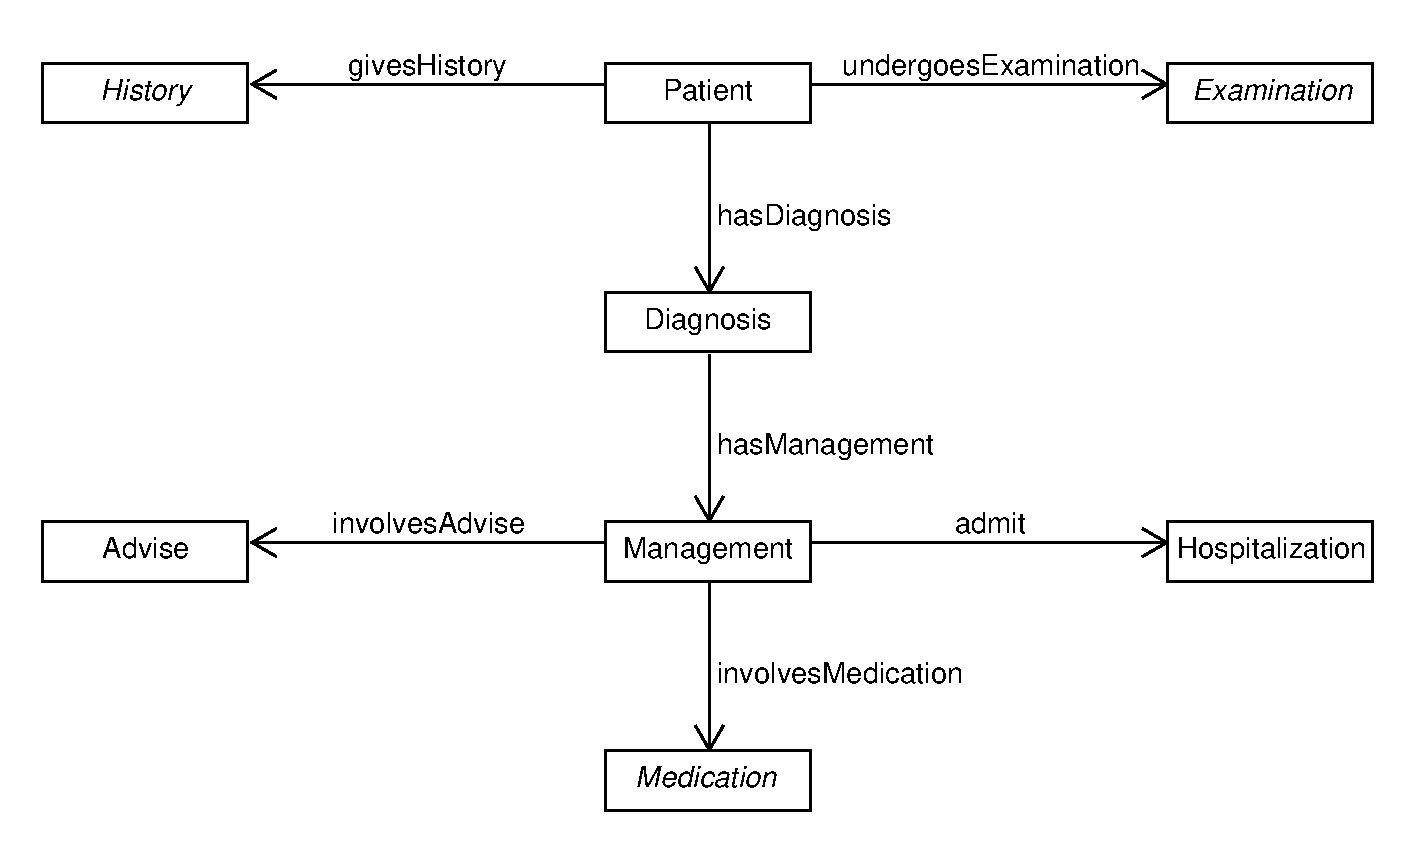
\includegraphics[scale=0.45]{SimpleEntityGraph}
\end{frame}


\begin{frame}[fragile]
\frametitle{Making scenarios, answer keys, distractions}
An instance of the entity model.
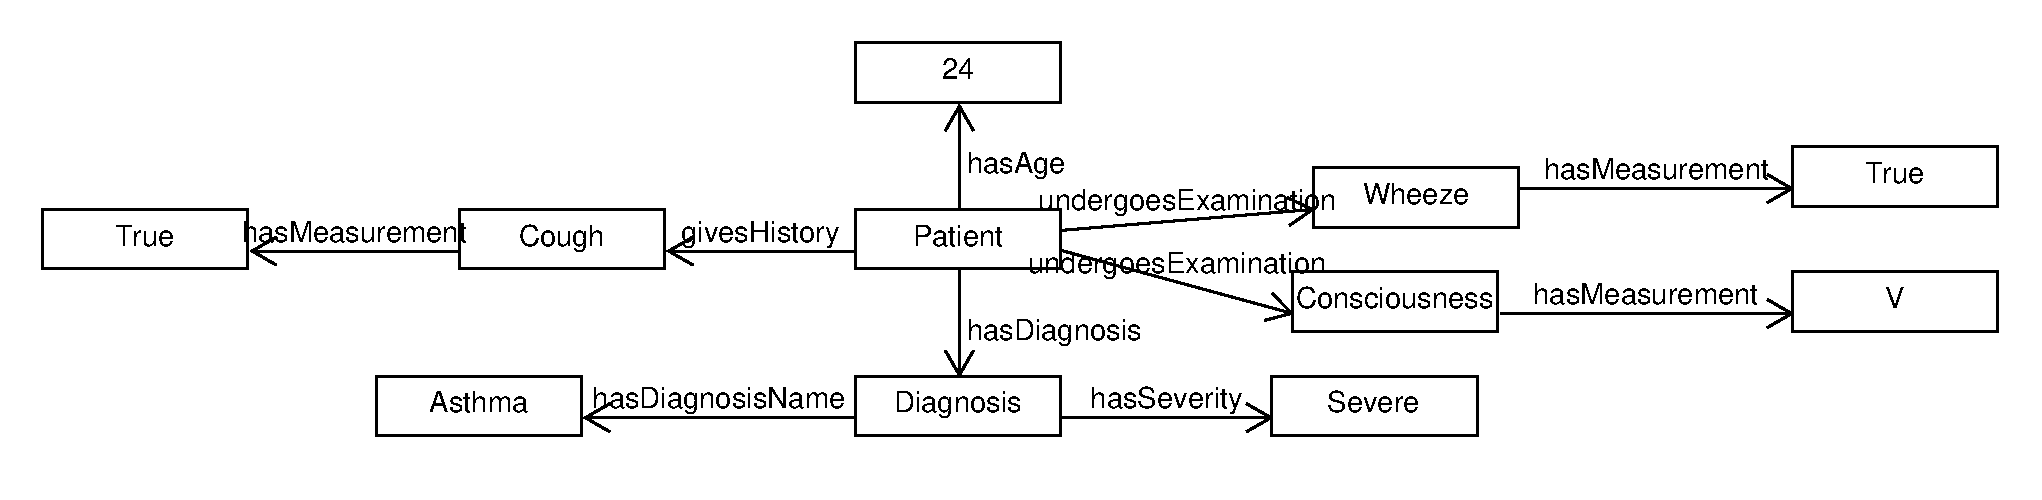
\includegraphics[scale=0.35]{EntityInstanceGraph}
\begin{semiverbatim}
A <\%Patient.hasAge.Age\%> old has arrived at the 
emergency clinic.  
She <\%Patient.givesHistory.Cough\%> 
<\%Patient.undergoesExamination.Wheeze\%>
<\%Patient.undergoesExamination.Consciousness\%>
\end{semiverbatim}
\end{frame}

\begin{frame}[fragile]
\frametitle{Making scenarios, answer keys, distractions}
An instance of the entity model.
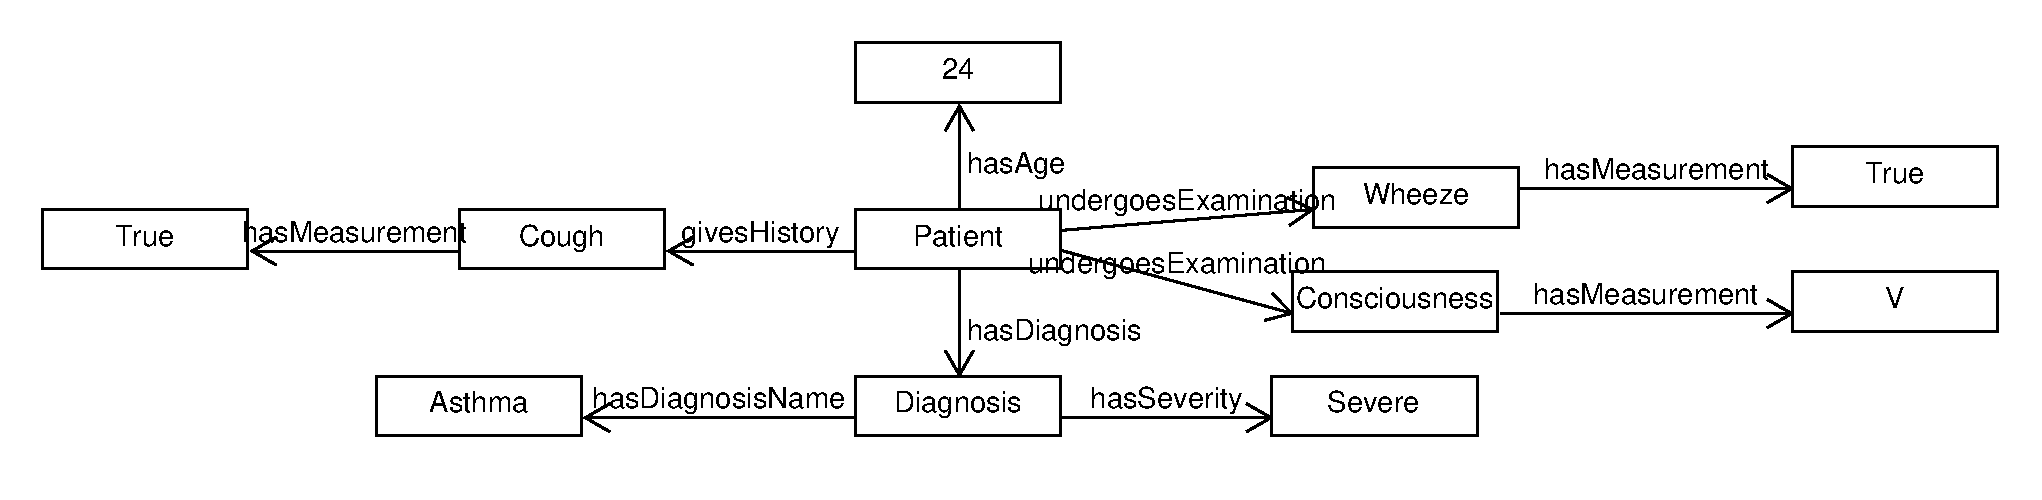
\includegraphics[scale=0.35]{EntityInstanceGraph}
\begin{semiverbatim}
	A 24 old has arrived at the 
	emergency clinic.  
	She True
	True
	V
\end{semiverbatim}
\end{frame}

\begin{frame}[fragile]
\frametitle{Making scenarios}
Adding presentation vertices to the instance.
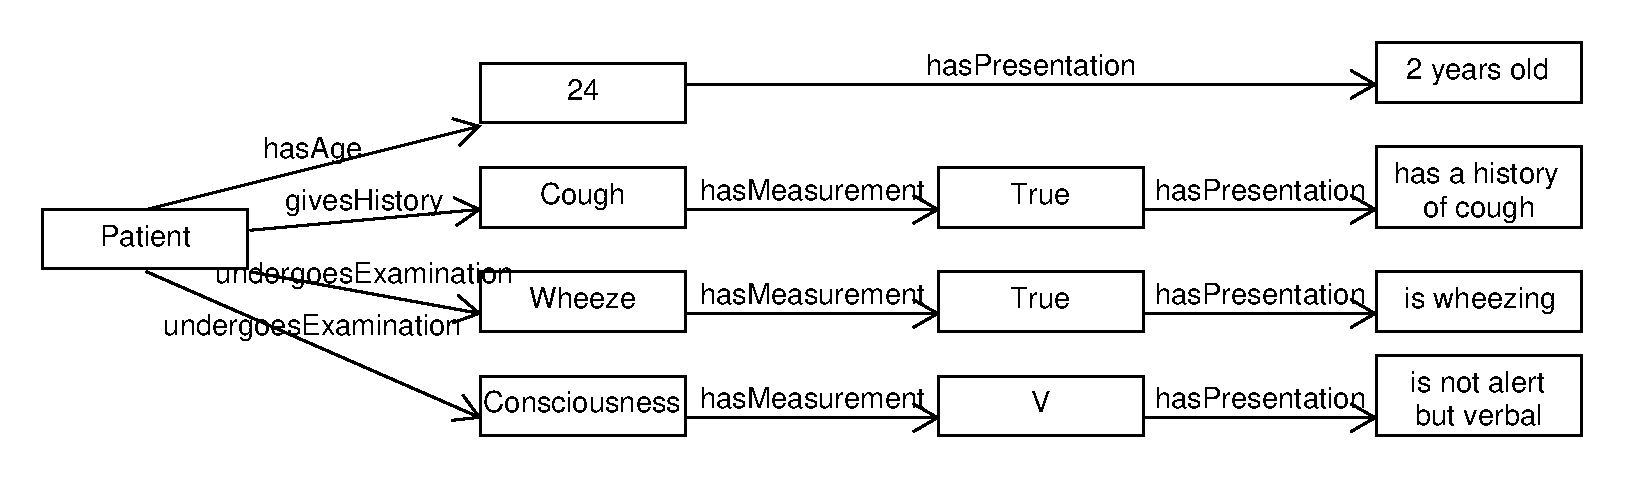
\includegraphics[scale=0.45]{PresentationEntityGraph}
\begin{semiverbatim}
	A 2 year old has arrived at the 
	emergency clinic.  
	She has a history of cough, 
	is wheezing
	and is not alert but verbal.
\end{semiverbatim}
\end{frame}

\begin{frame}{Entity- and workflow model working together}
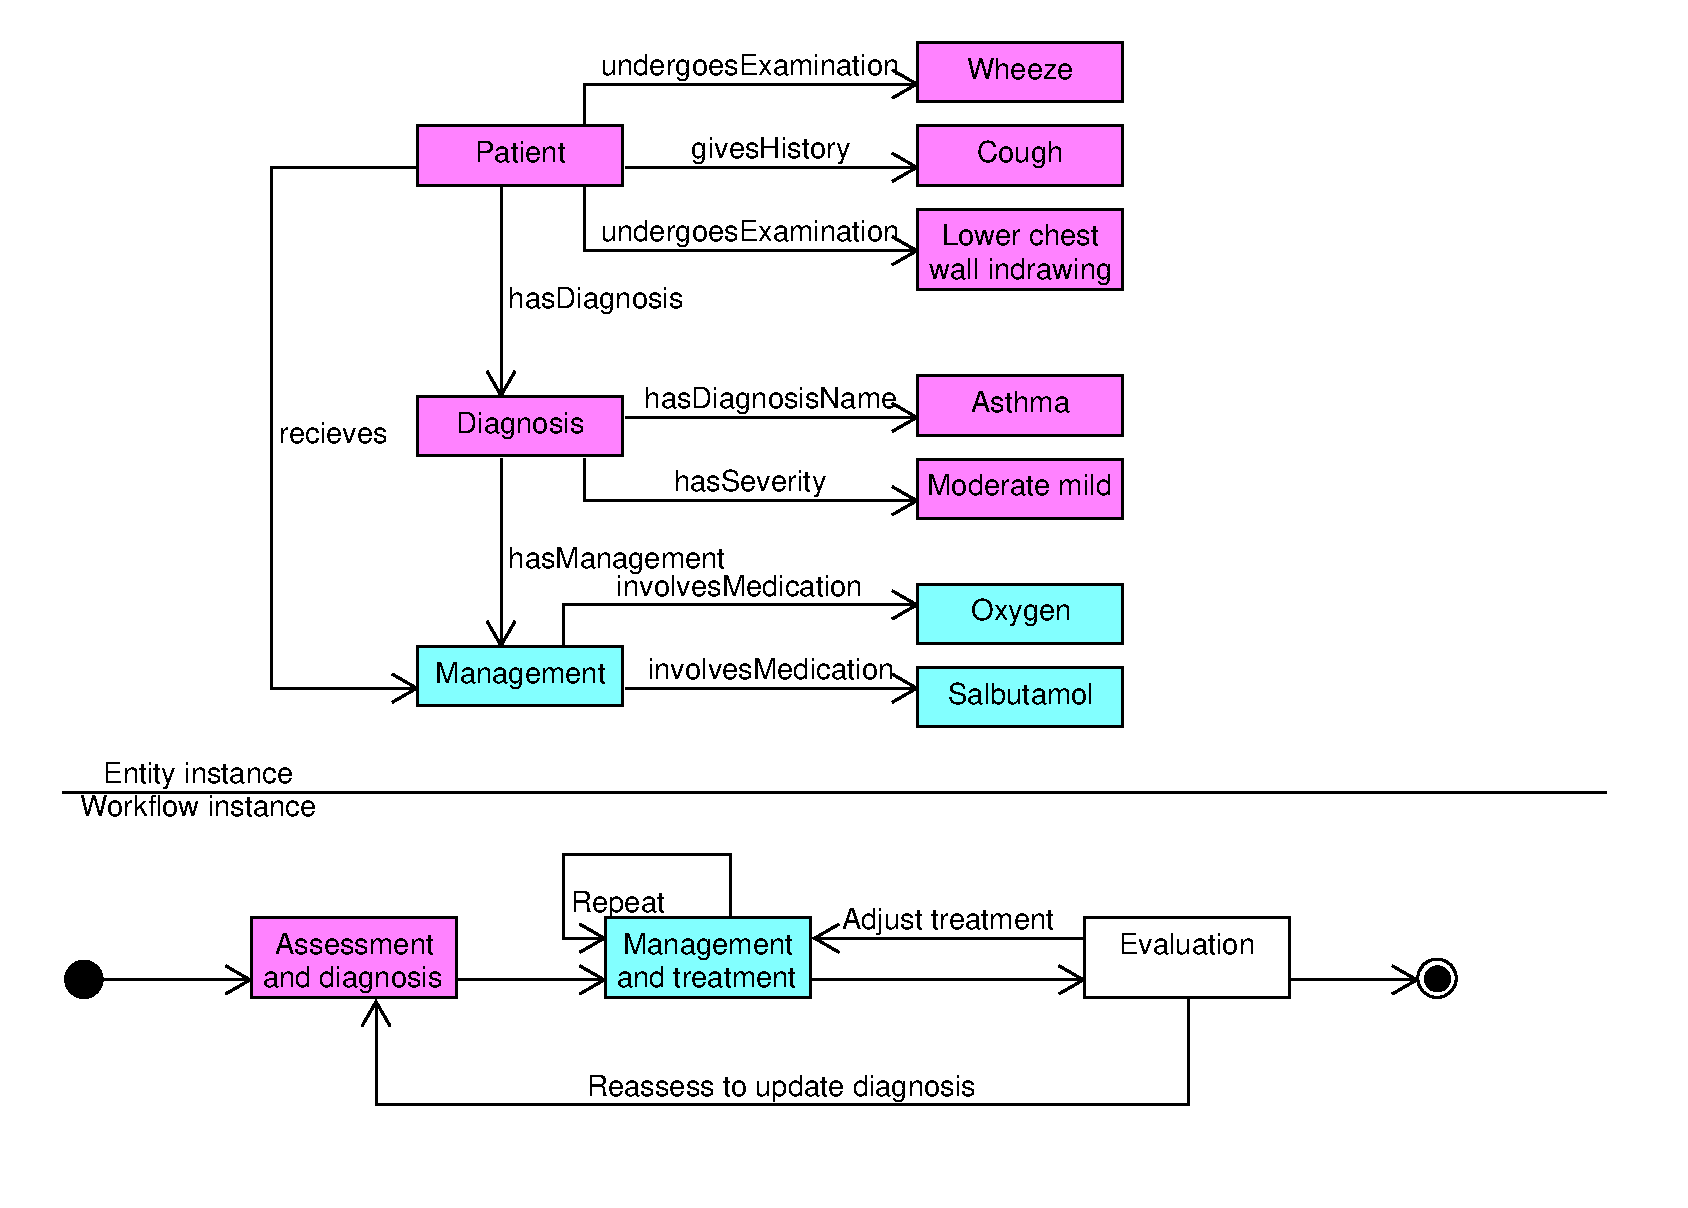
\includegraphics[scale=0.40]{Integrated1}
\end{frame}

\begin{frame}{Entity- and workflow model working together	}
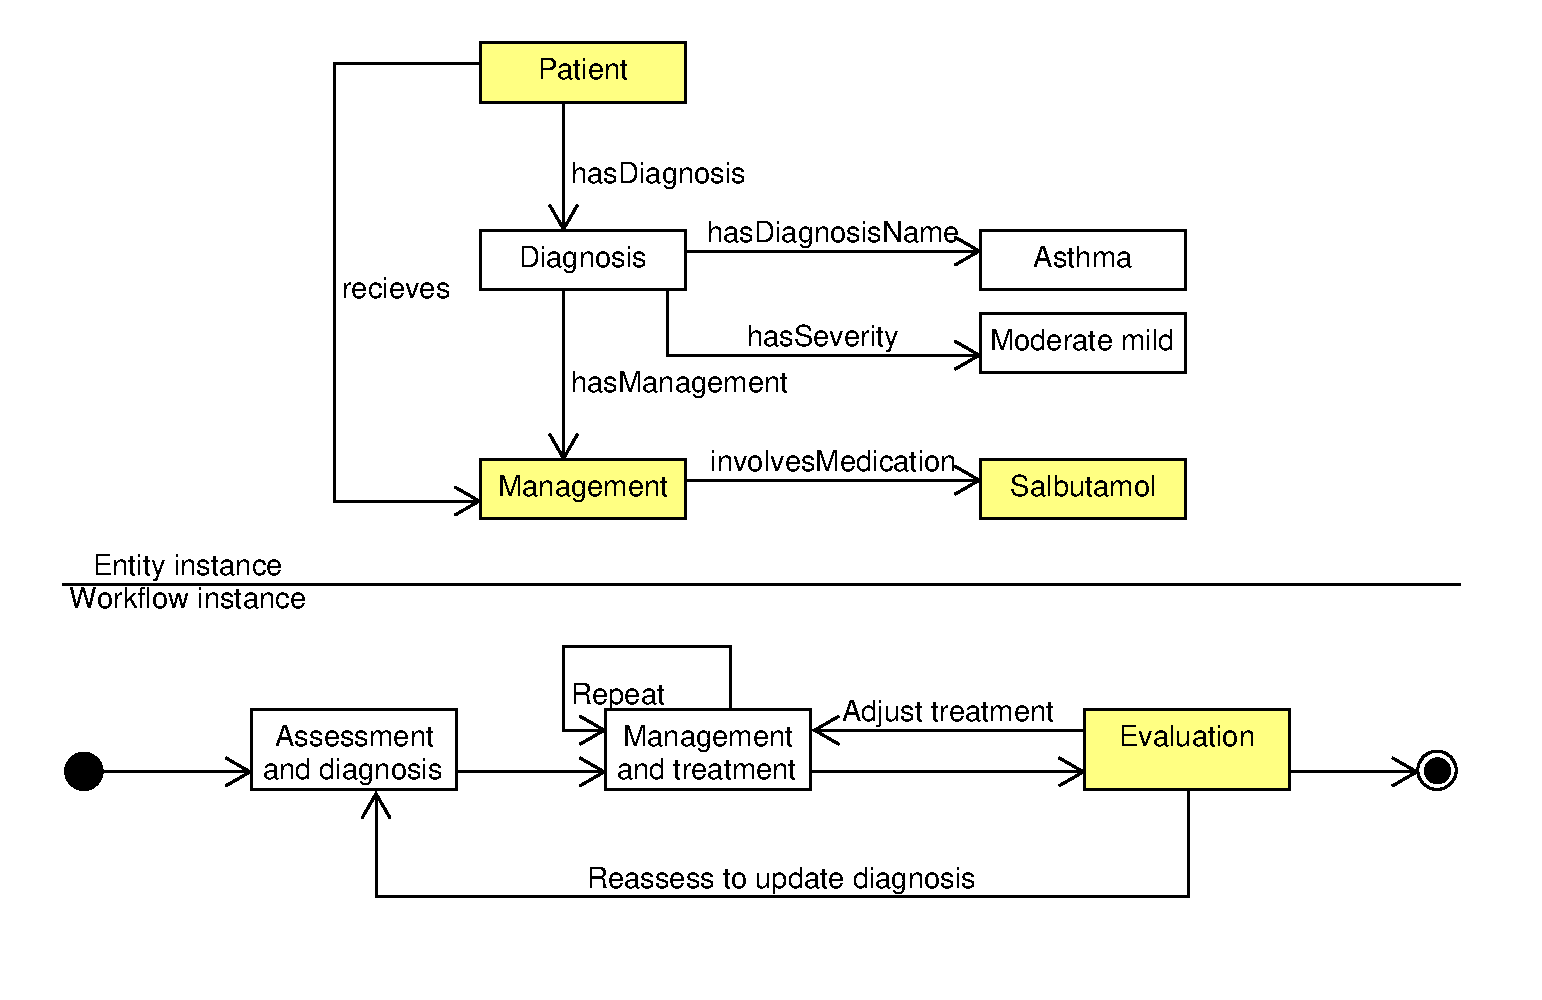
\includegraphics[scale=0.45]{Integrated2}
\end{frame}

\begin{frame}{Dynamic Content Management}
\begin{itemize}
	\item \textbf{Adaptive learning:} Students will solve problems which are suited to their level of knowledge.
	\item \textbf{Flexibility in the learning process:} As long as the students follow the knowledge dependencies, they can go through the learning material in many different ways.
\end{itemize}
\end{frame}


\begin{frame}{Dynamic Content Management}
\begin{itemize}
	\item Split the learning content into atomic units of knowledge.
	\item Build up courses (quizzes) by selecting and organizing the knowledge units.
	\item Identify dependencies between the knowledge units.
\end{itemize}
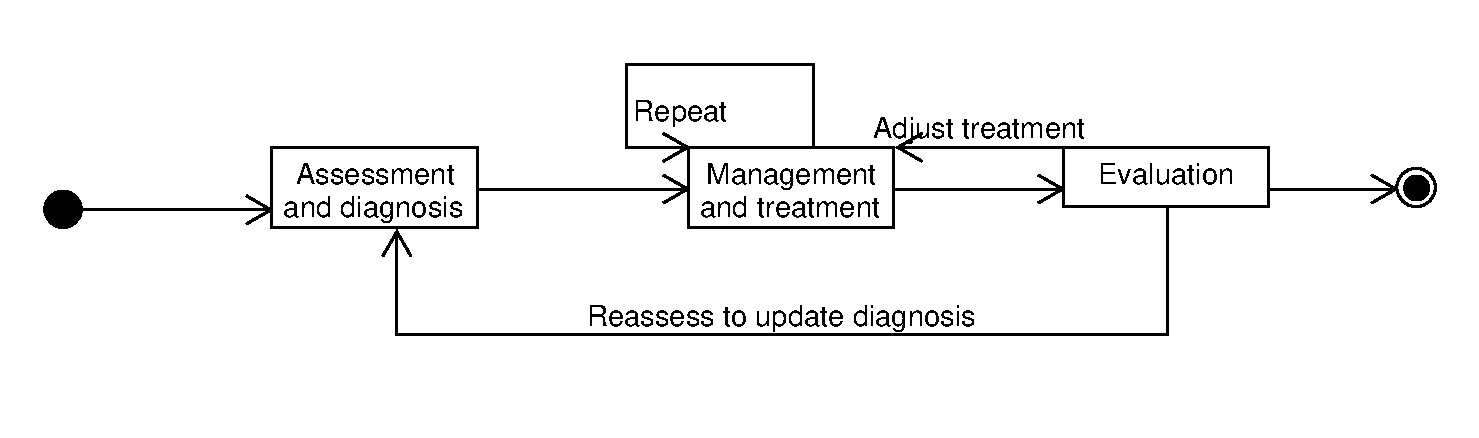
\includegraphics[scale=0.44]{WorkflowGraph}
%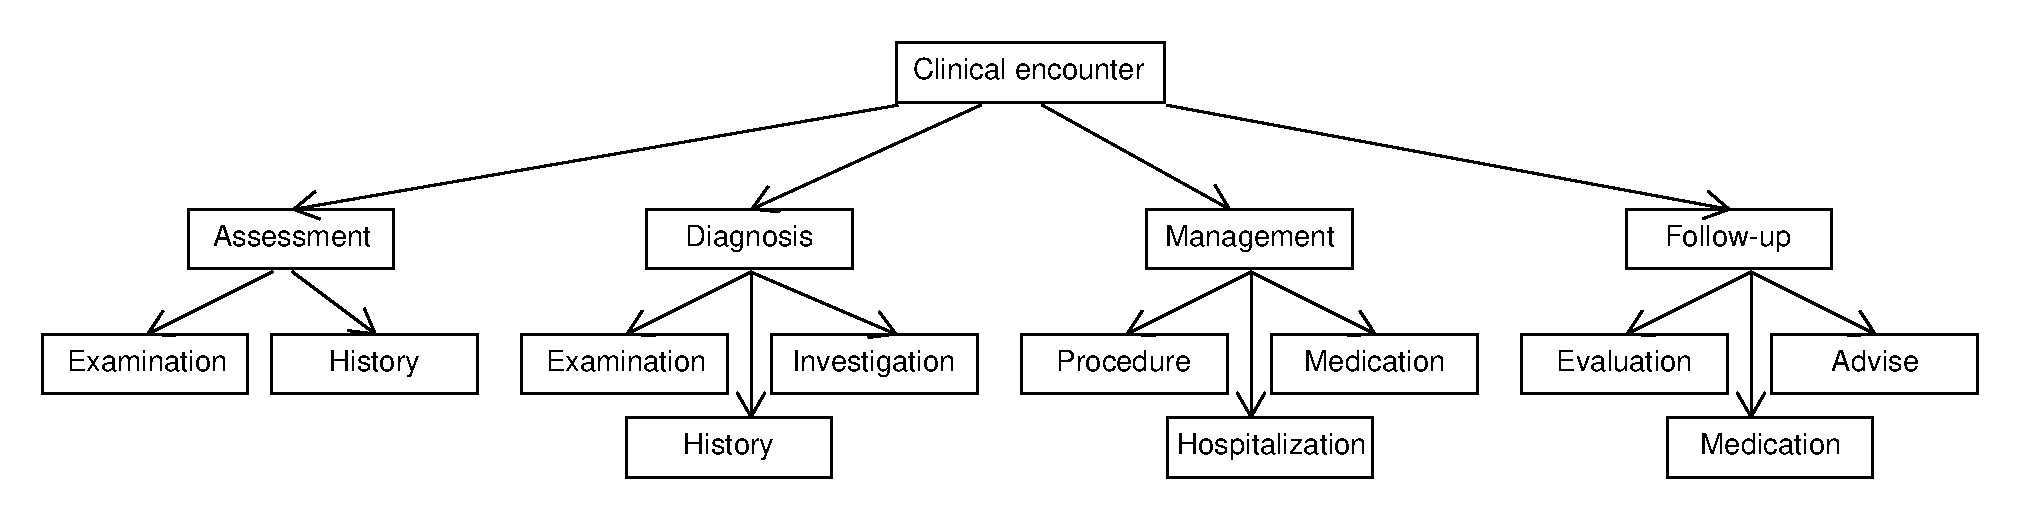
\includegraphics[scale=0.36]{KnowledgeMap}
\end{frame}

\begin{frame}{Dynamic Content Management}
\textbf{Knowledge Map} shows the dependencies in the learning process. 
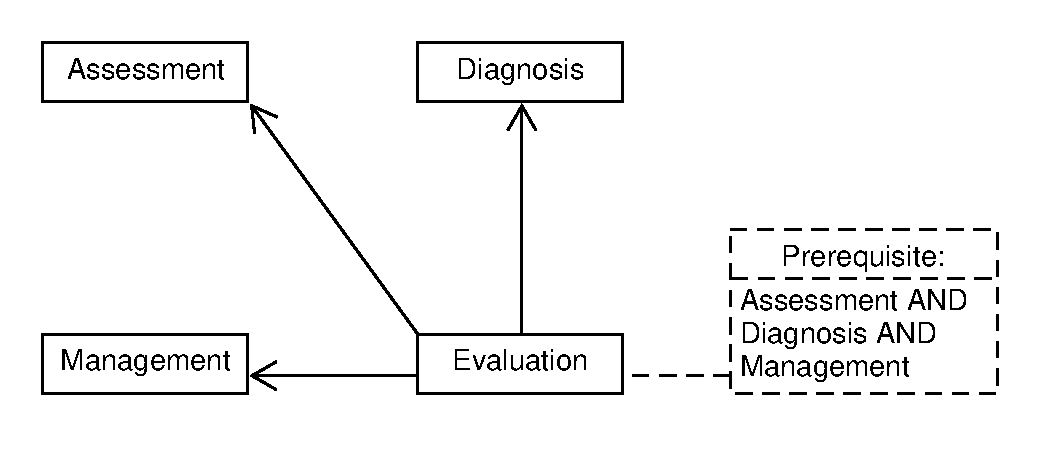
\includegraphics[scale=0.5]{Knowledge}
\end{frame}

\begin{frame}{Dynamic Content Management}
\begin{table}[h!]
\begin{tabular}{|m{2em}|m{6em}|m{6em}|m{6em}|m{6em}|}
	\hline
	 Level & Assessment & Diagnosis & Management & Evaluation \\
	\hline
	1  & Factual & Factual & Factual & - \\
	2 & Scenario & Scenario & Scenario & Scenario \\
	3 & Detailed scenario  & Detailed scenario & Detailed scenario & Detailed scenario \\
	\hline
\end{tabular}
\end{table}
\begin{itemize}
	\item Learning map shows all paths through the learning material.
	\item Student map shows one student's path in the learning map.
\end{itemize}
\end{frame}


\begin{frame}{Demonstration}
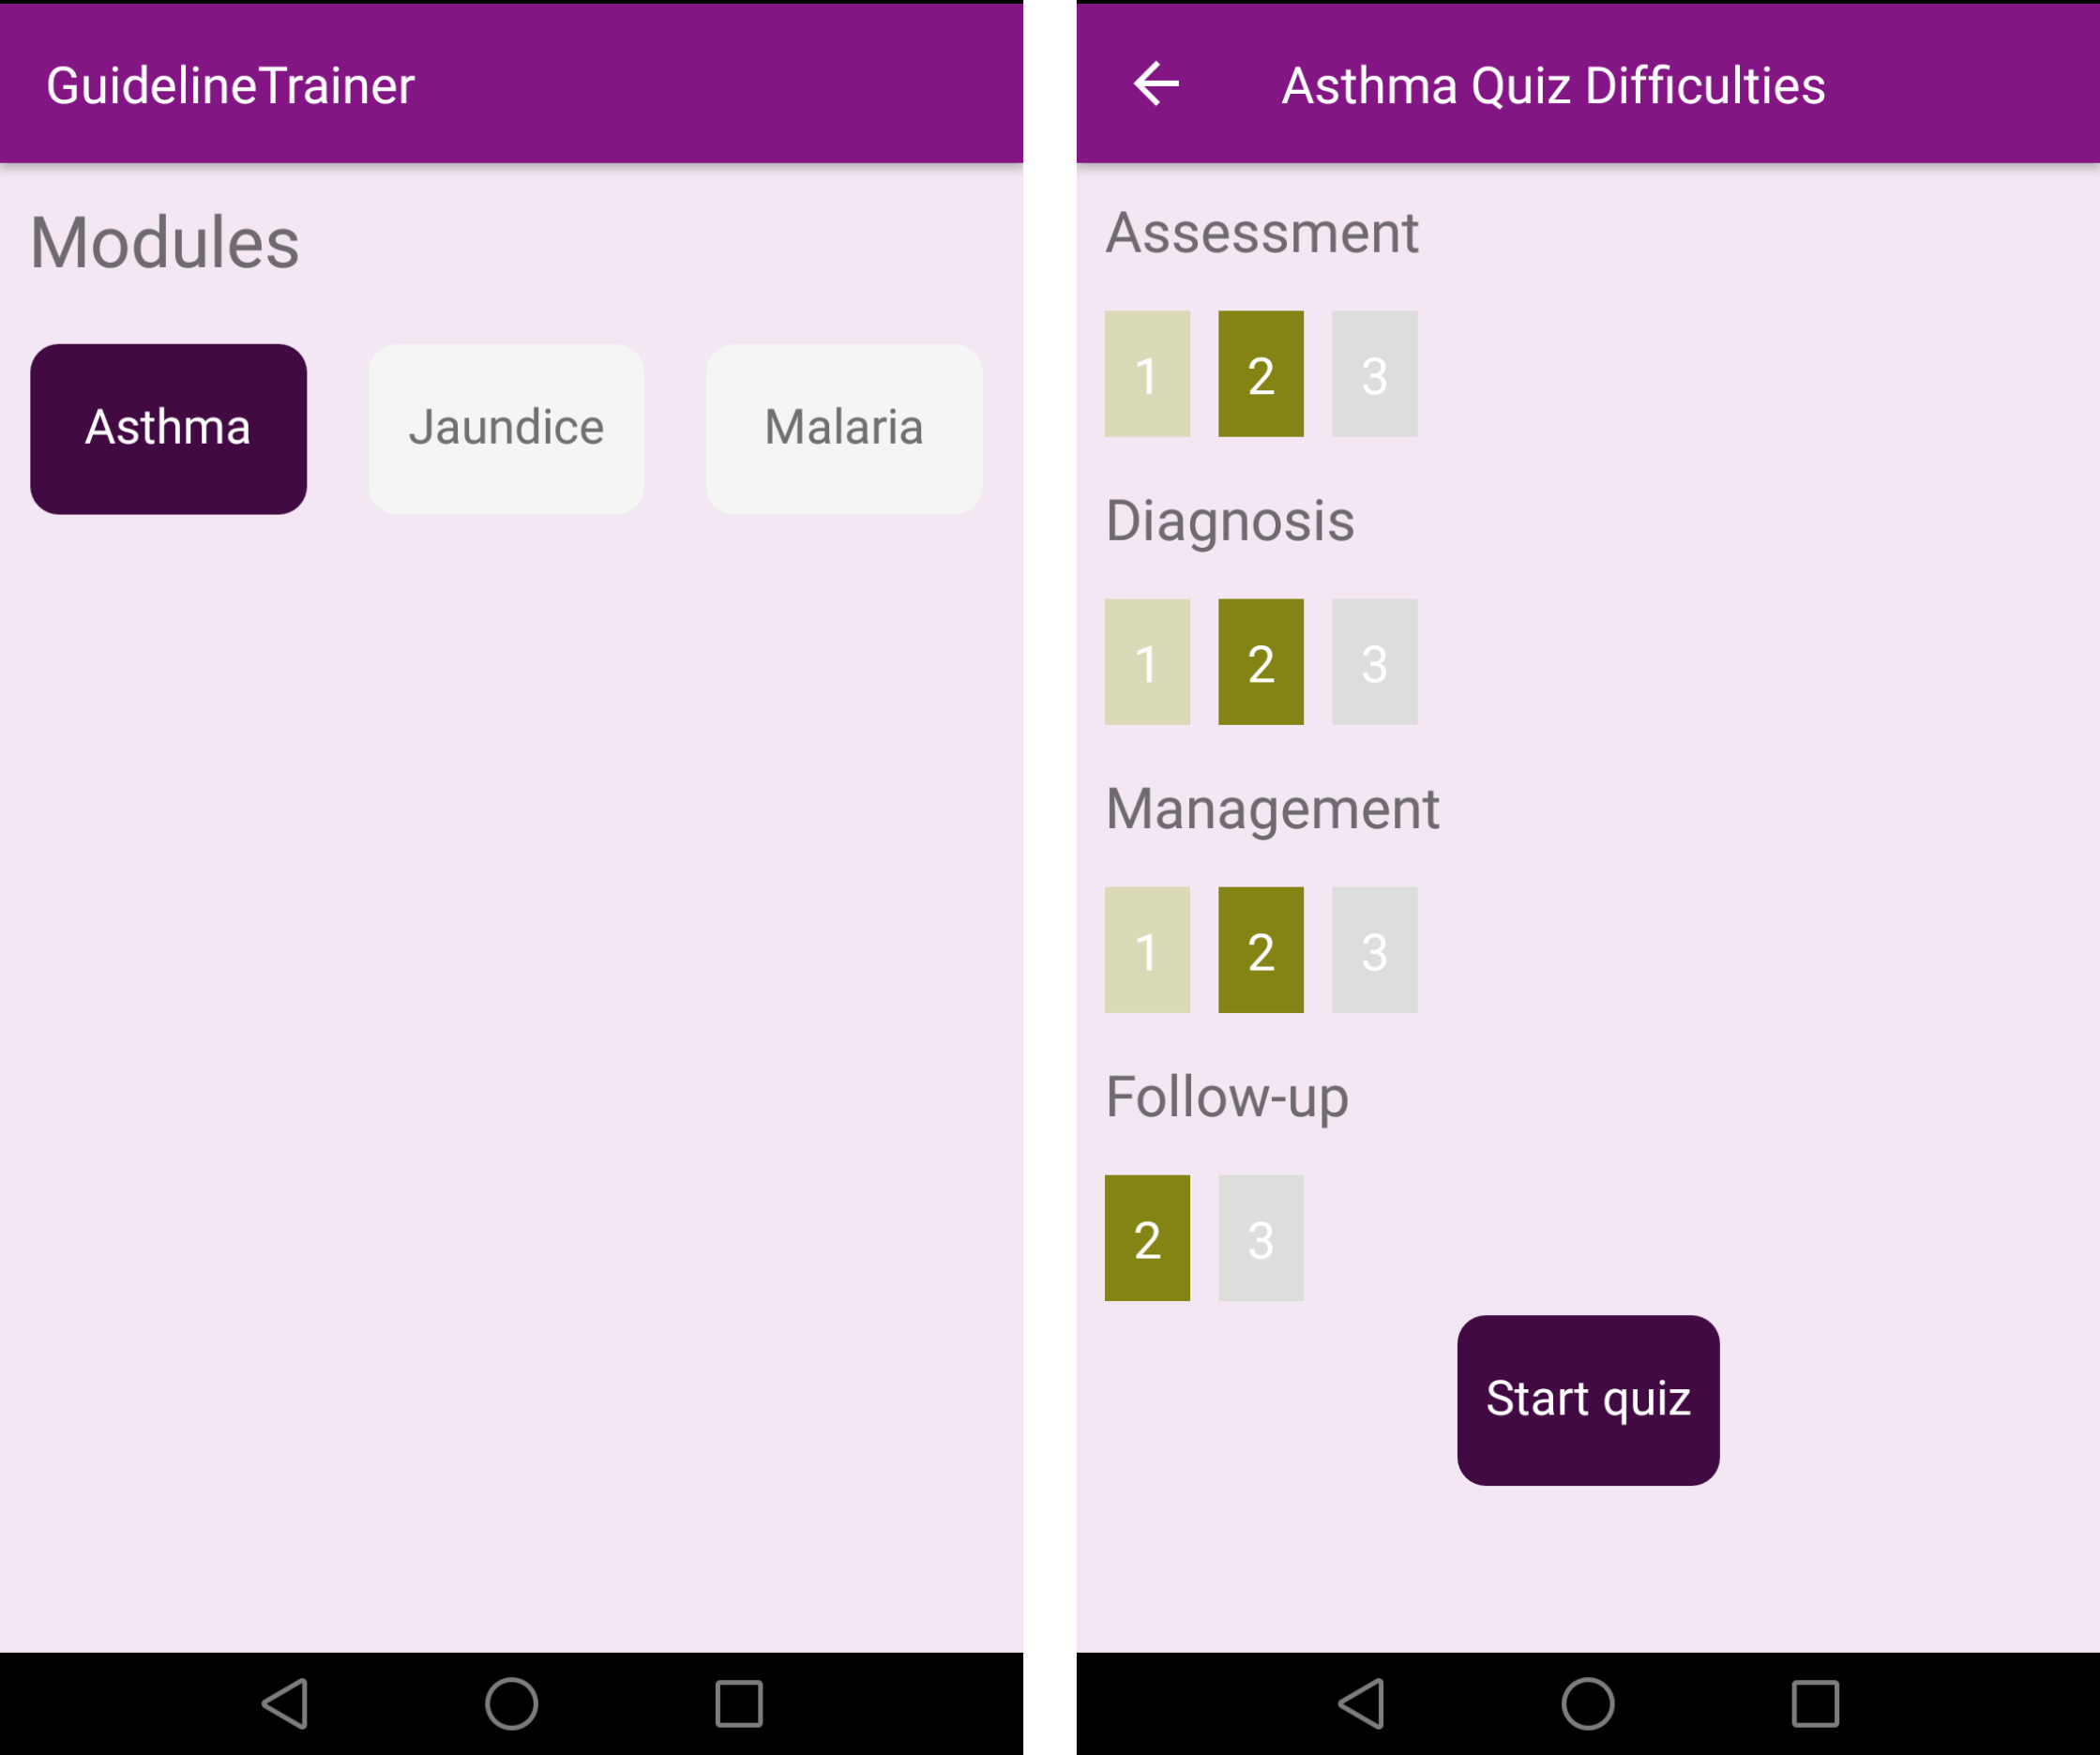
\includegraphics[scale=0.16]{Montage1}
\end{frame}
\begin{frame}{Demonstration}
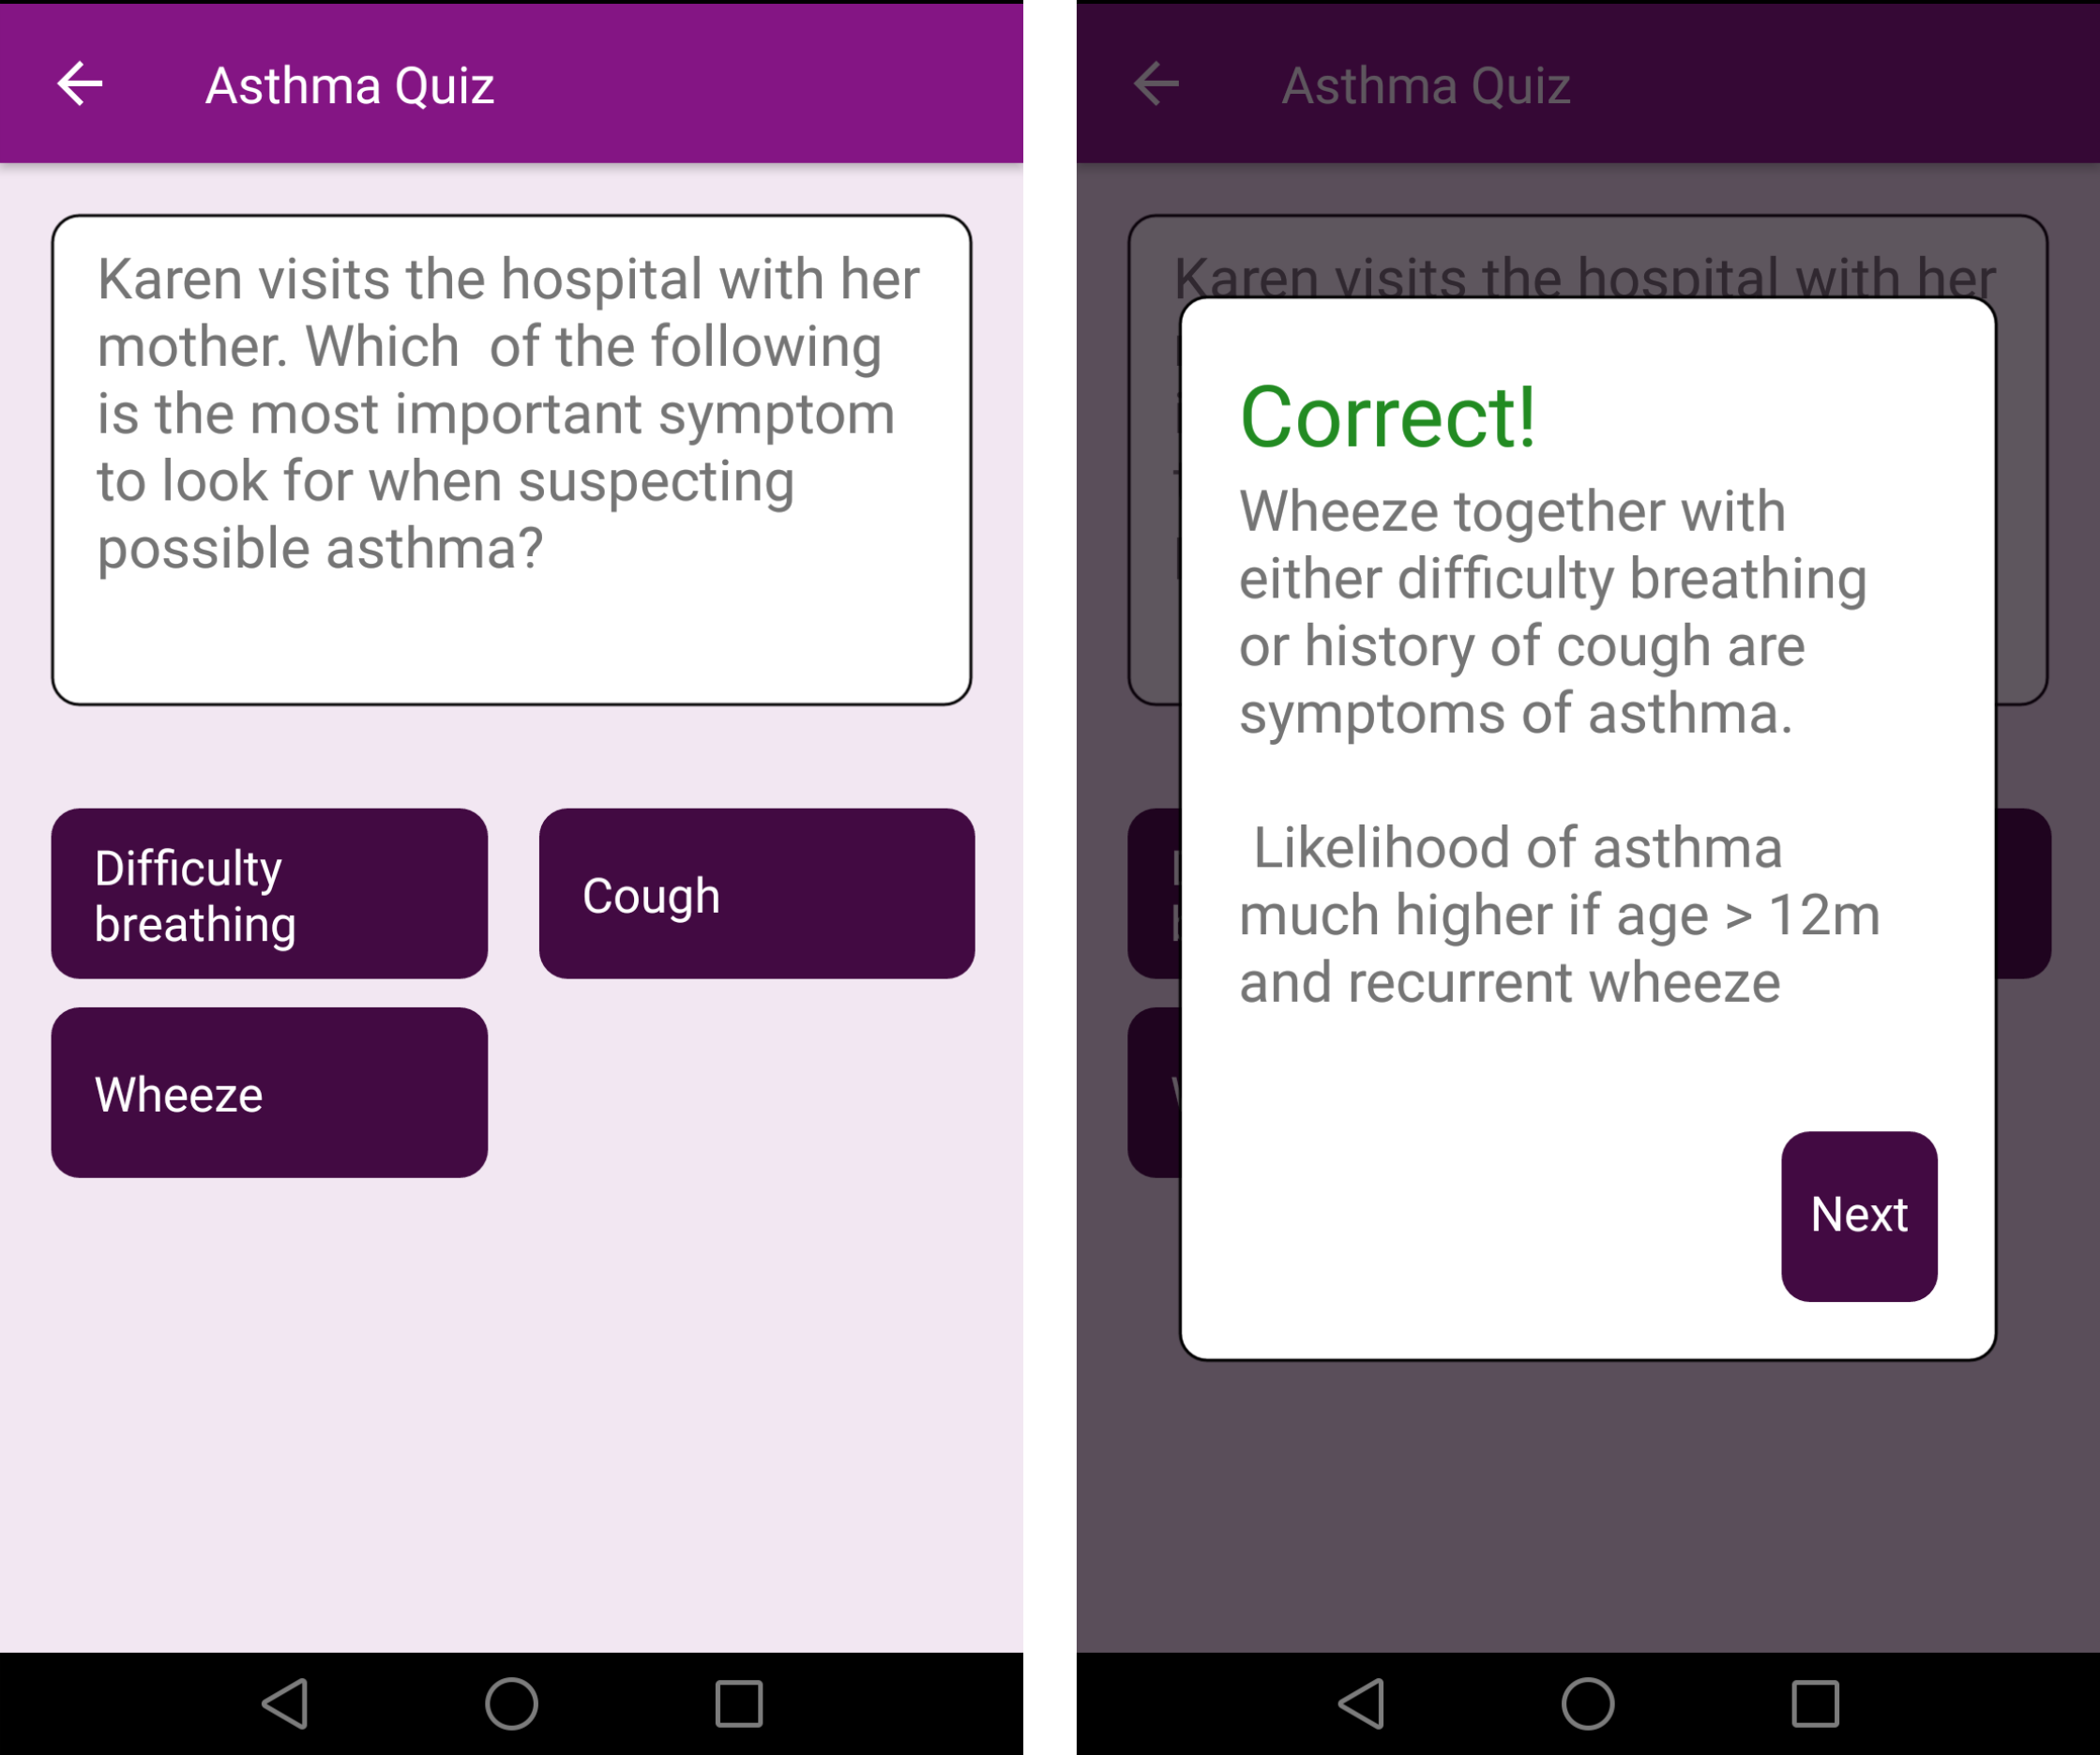
\includegraphics[scale=0.16]{Montage2}
\end{frame}
\begin{frame}{Demonstration}
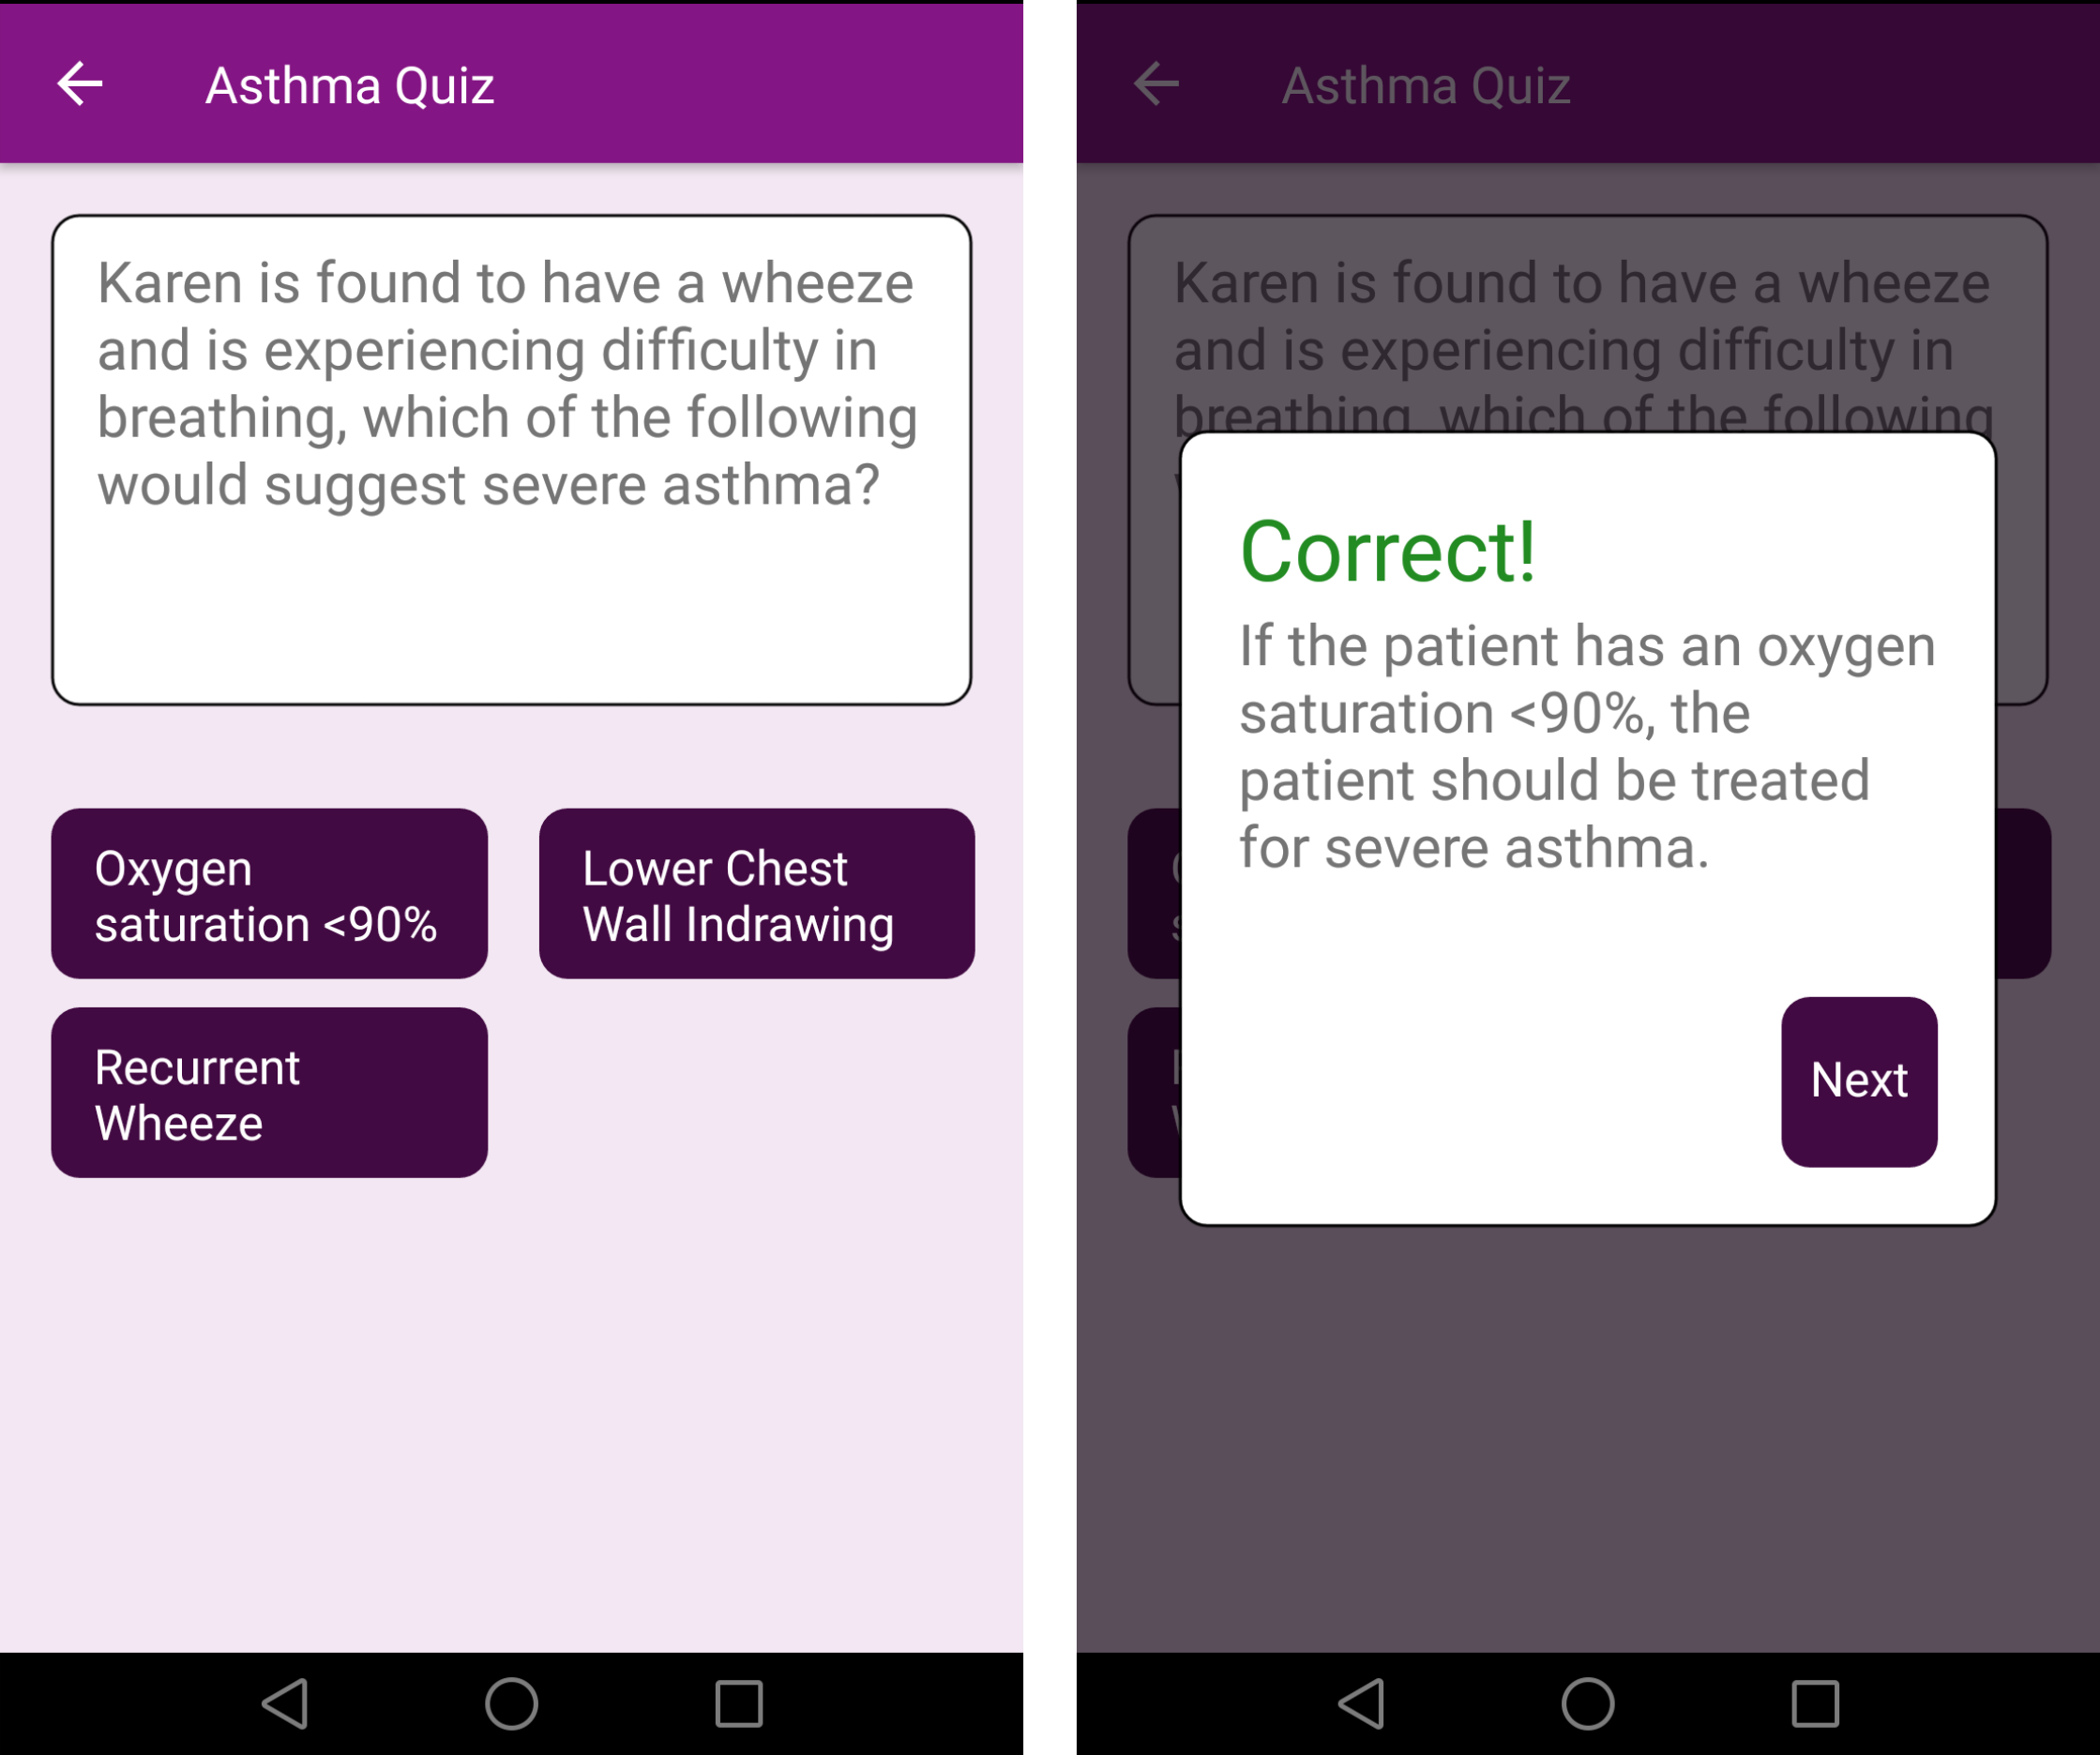
\includegraphics[scale=0.16]{Montage3}
\end{frame}
\begin{frame}{Demonstration}
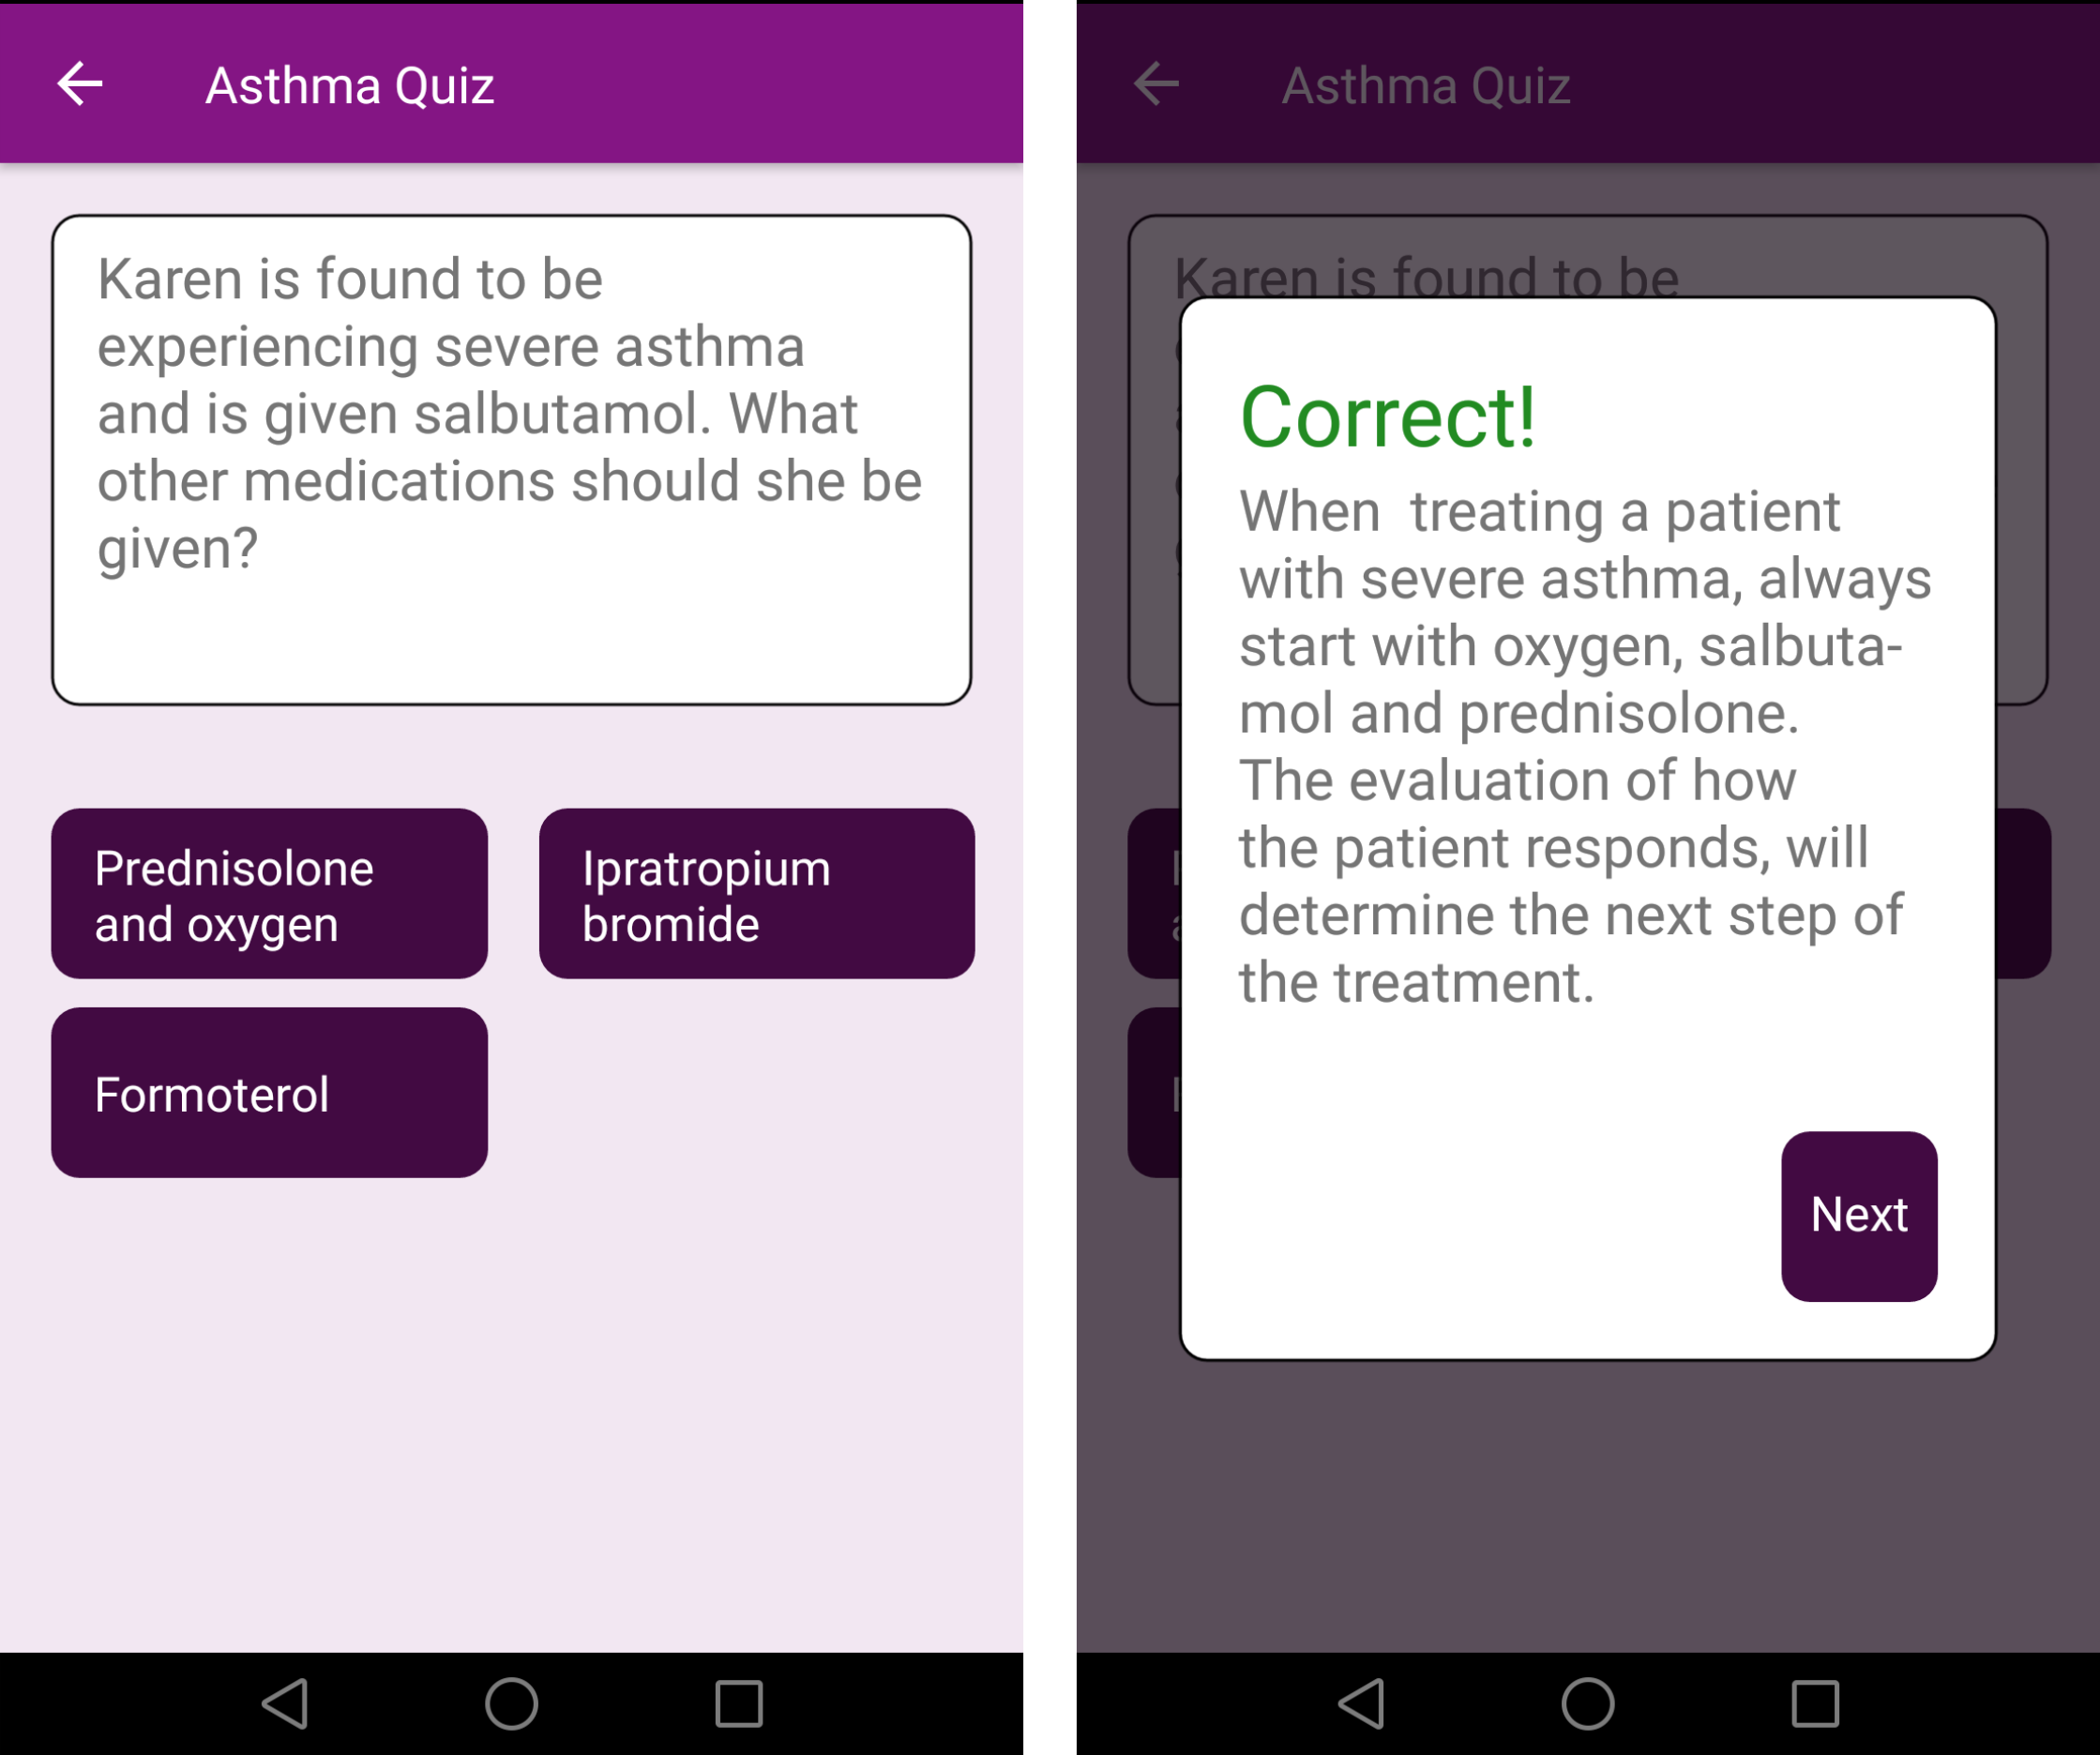
\includegraphics[scale=0.16]{Montage4}
\end{frame}
\begin{frame}{Demonstration}
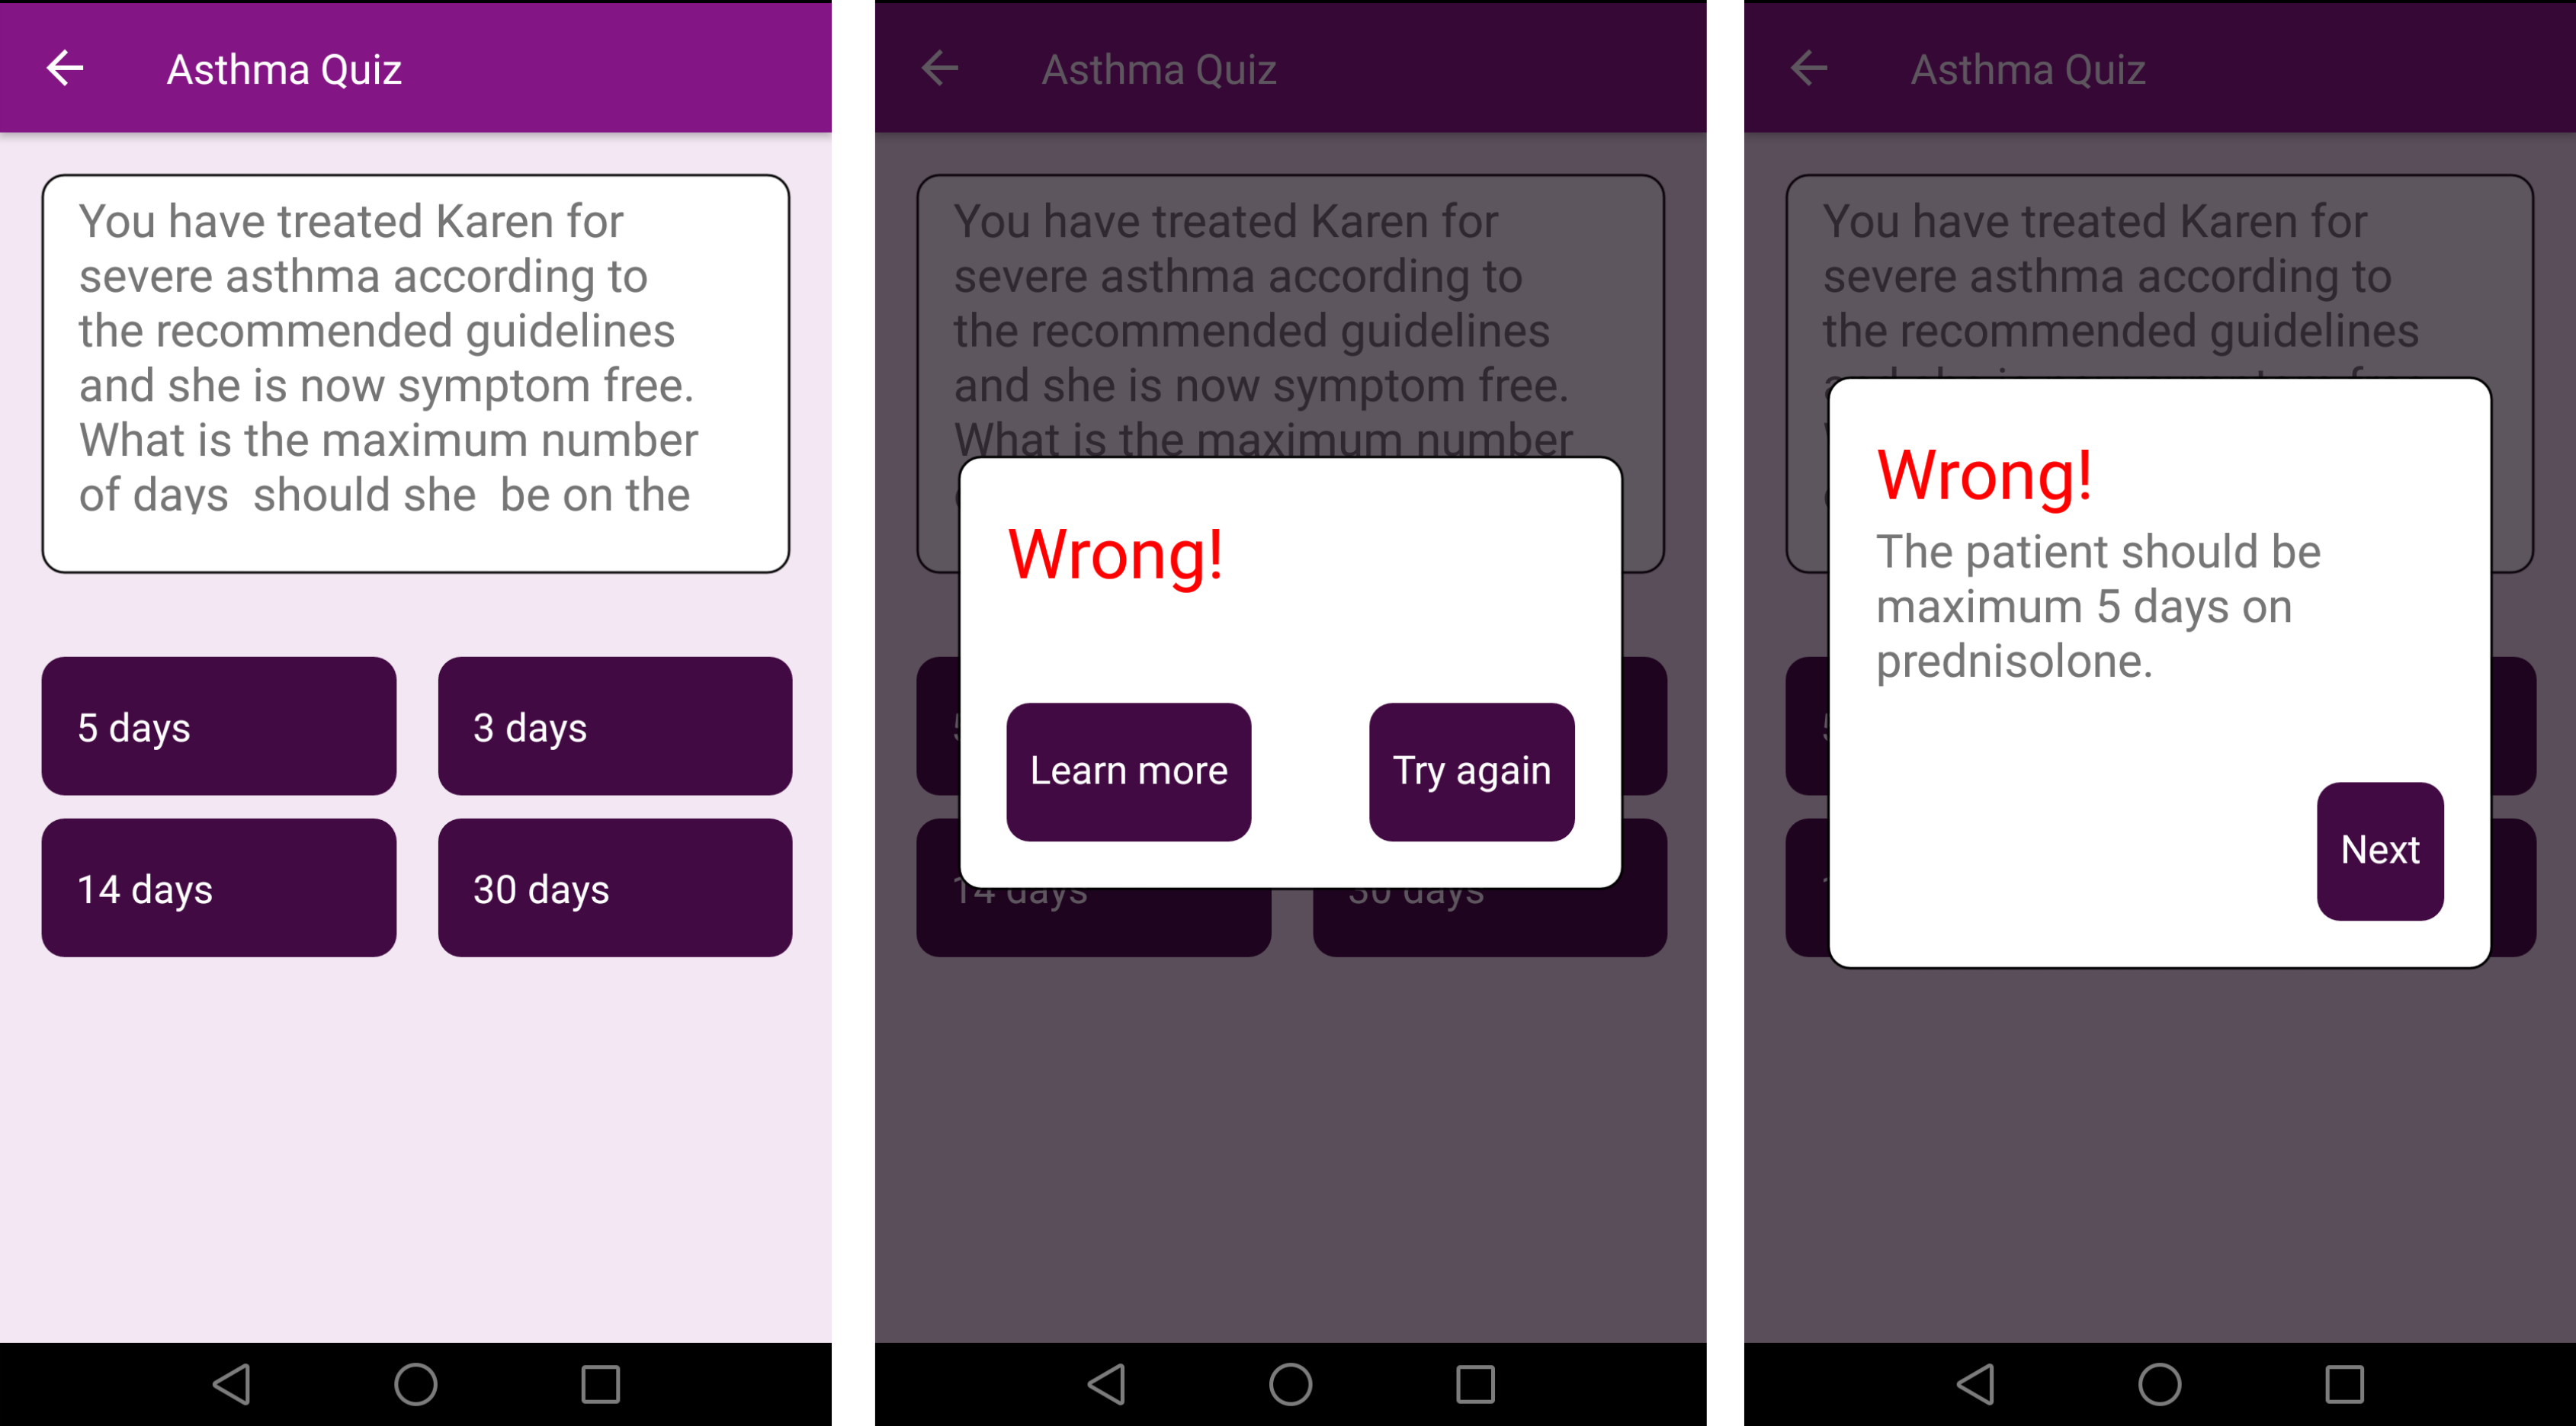
\includegraphics[scale=0.14]{Montage5}
\end{frame}
\begin{frame}{Demonstration}
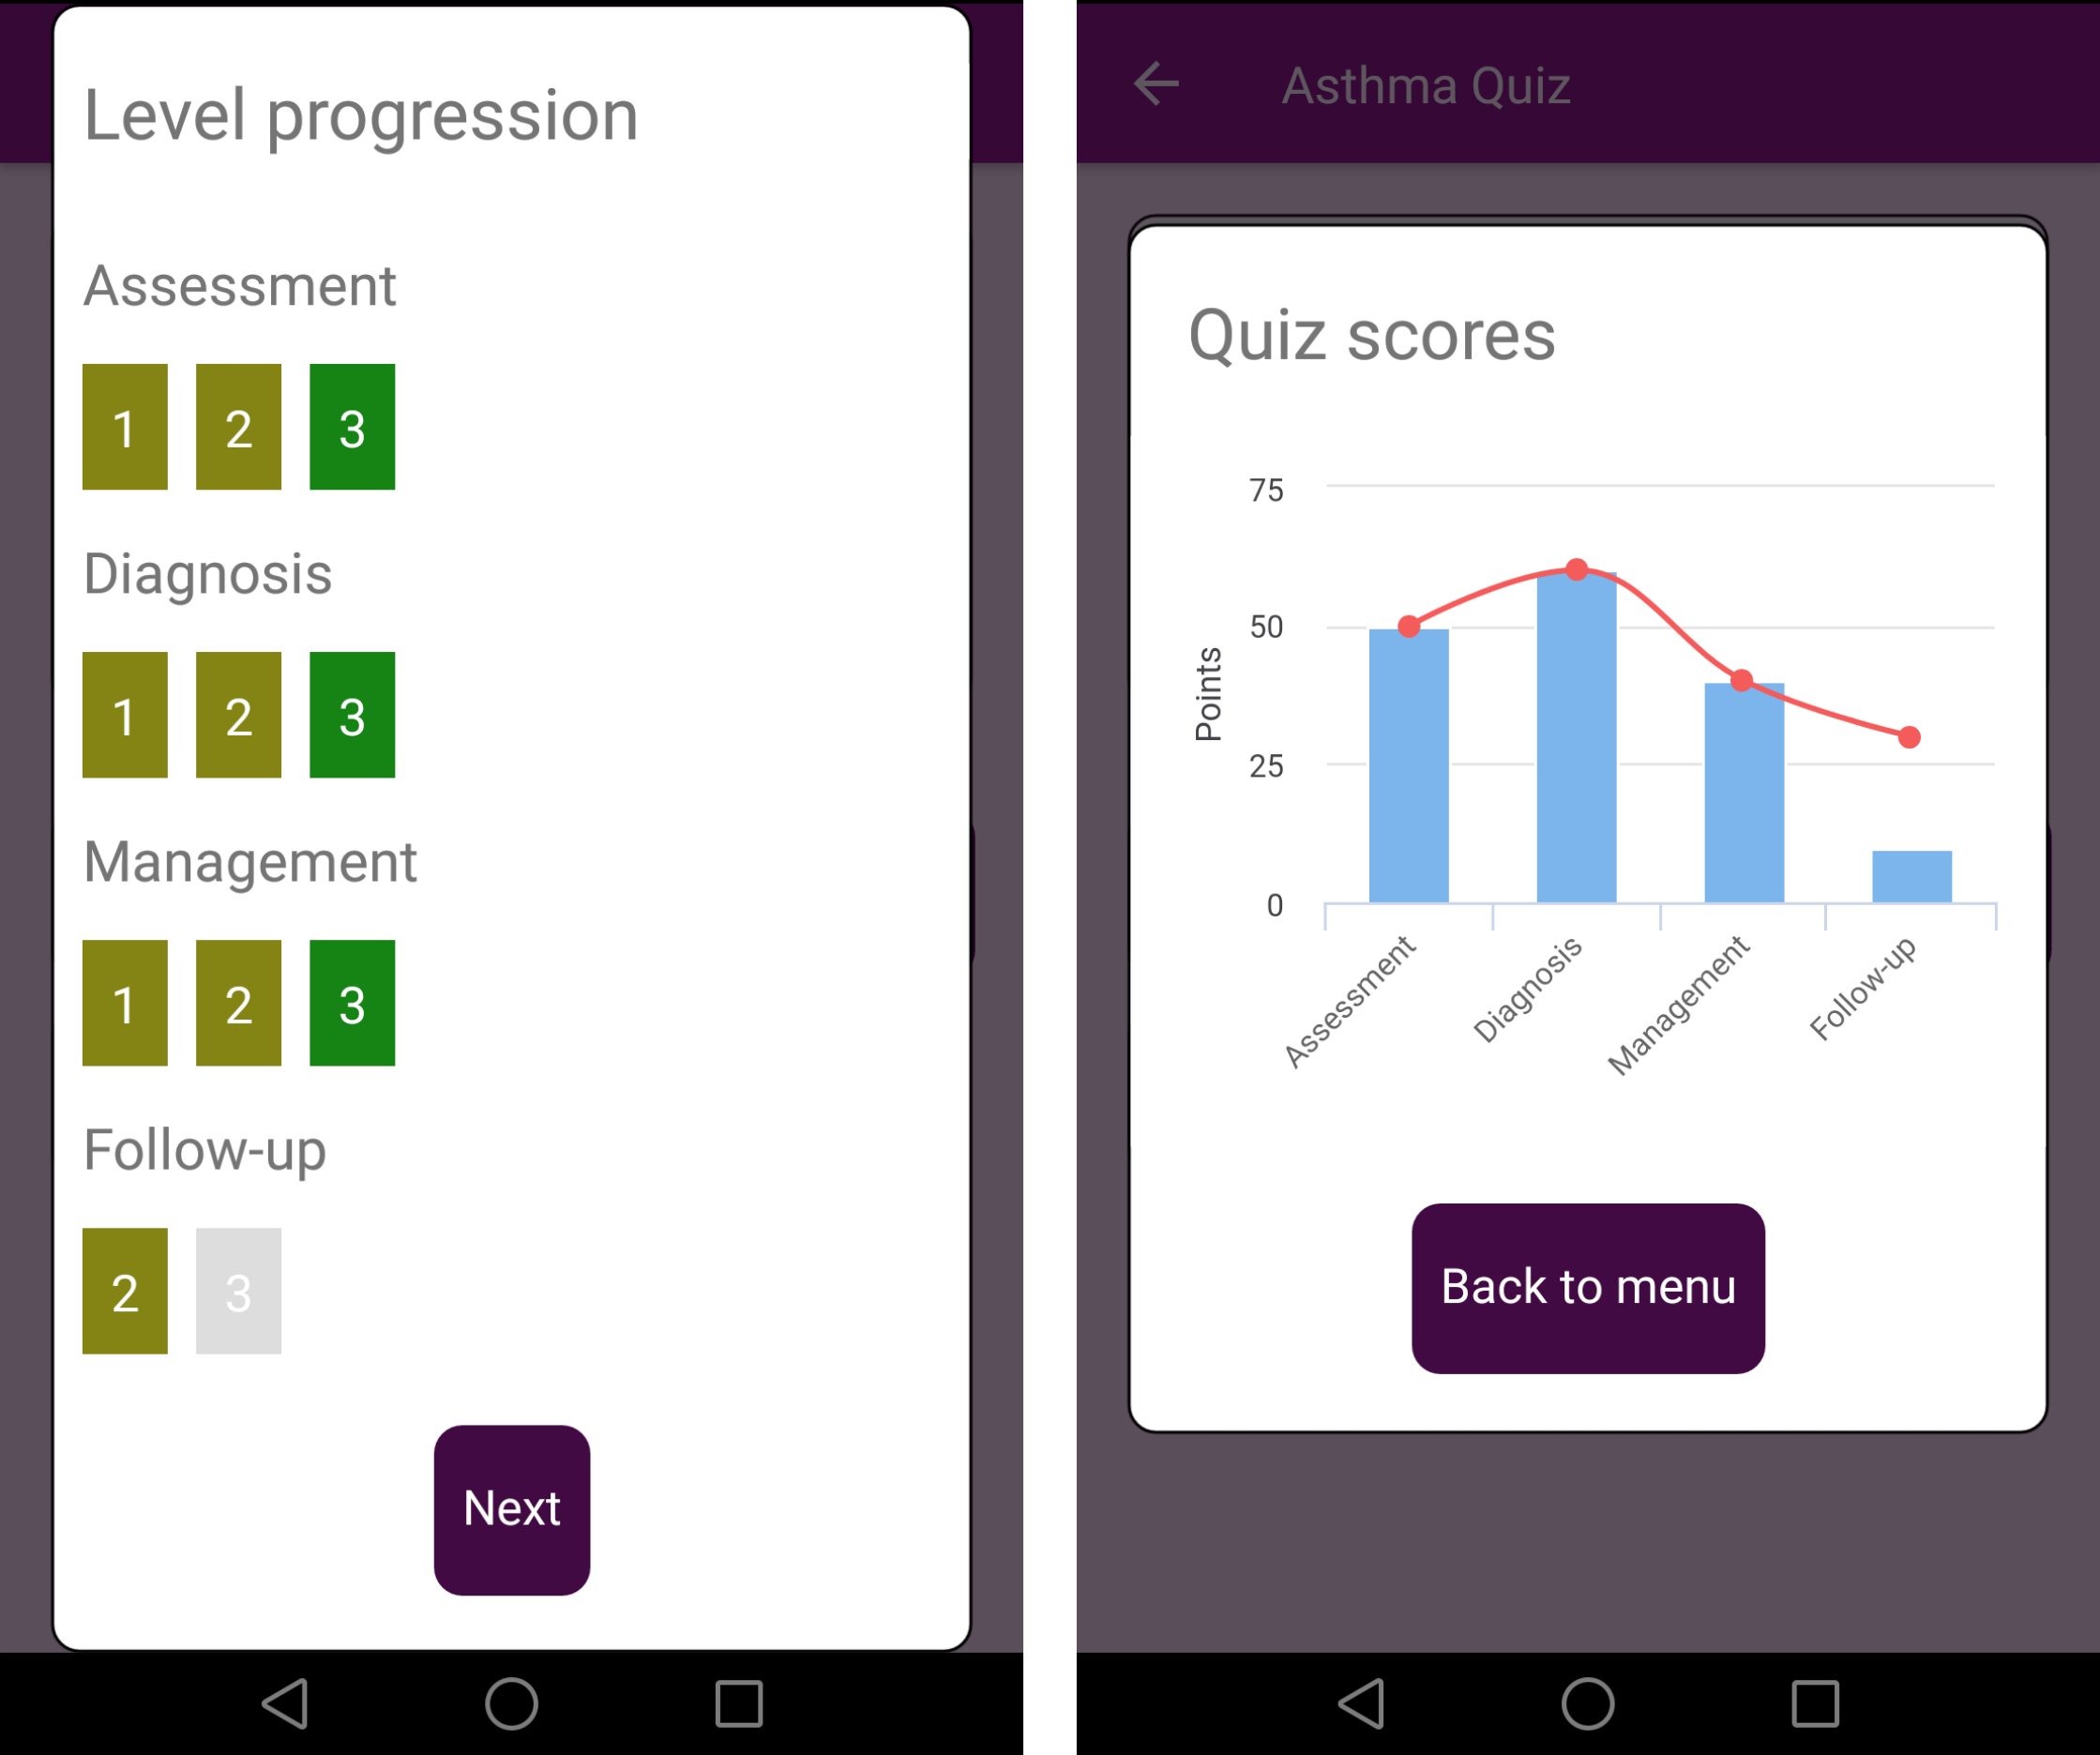
\includegraphics[scale=0.16]{Montage6}
\end{frame}

\begin{frame}{Modelling paediatric pneumonia}
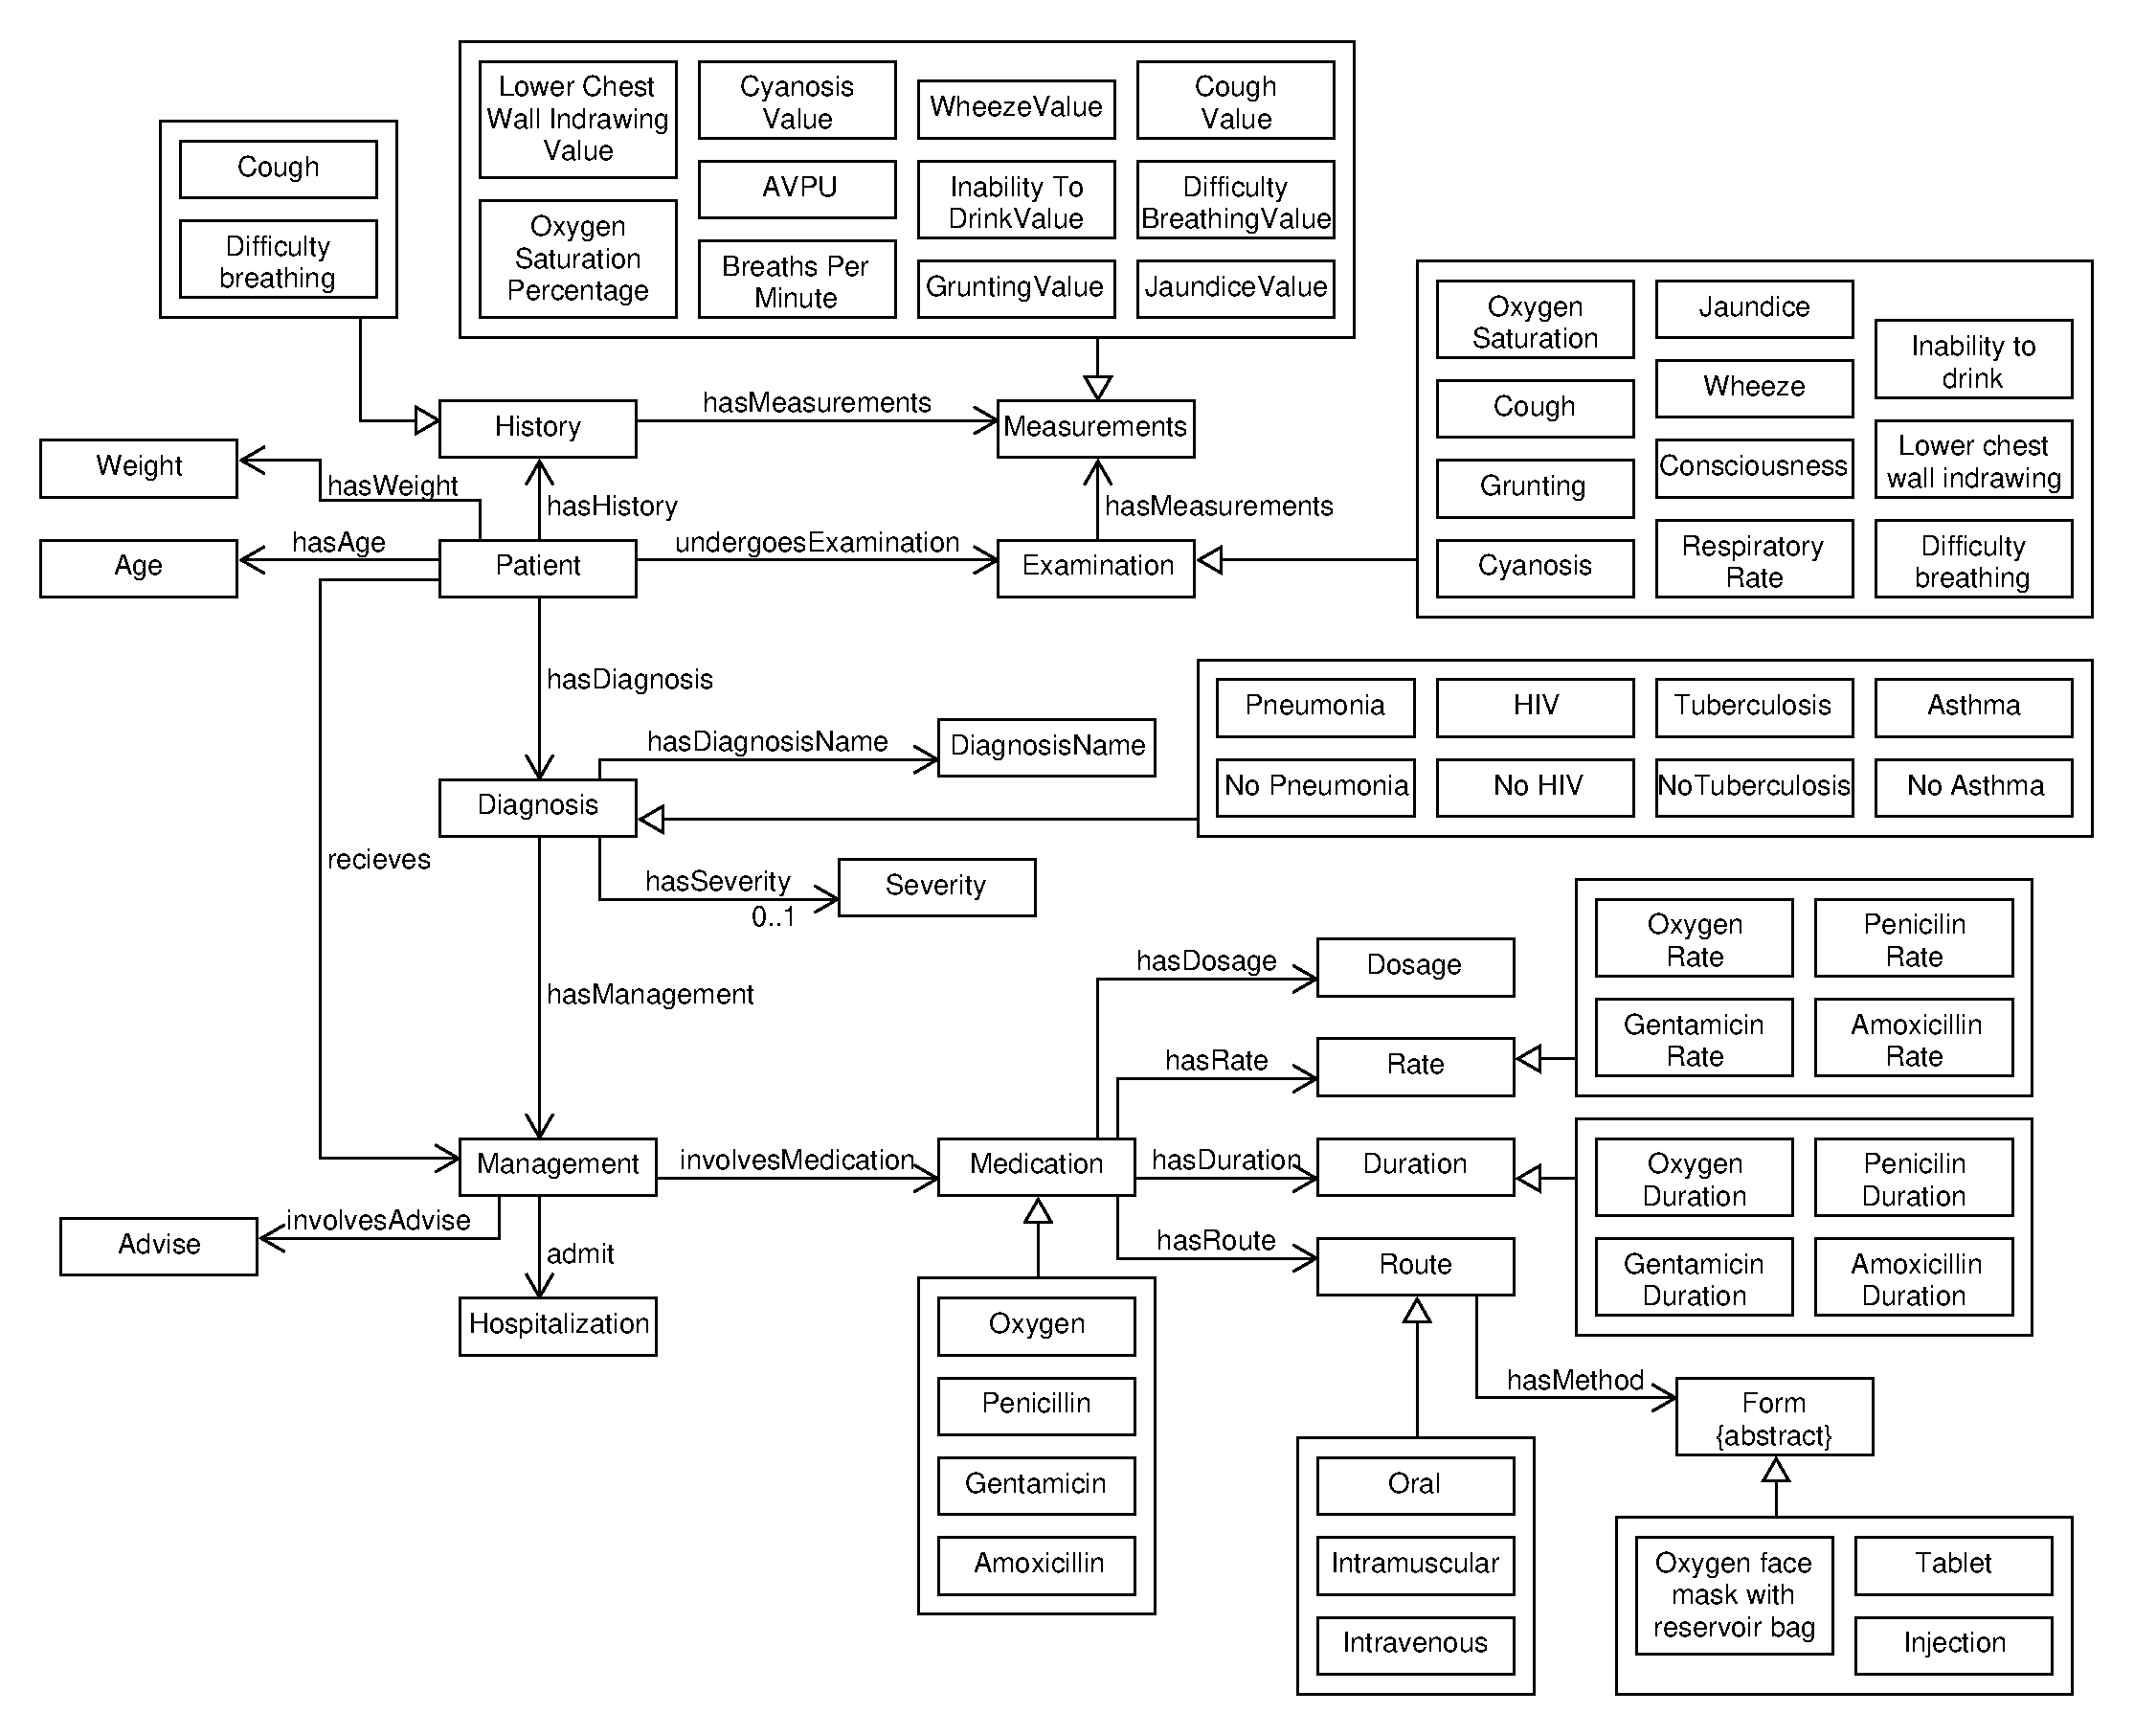
\includegraphics[scale=0.27]{Pneumonia}
\end{frame}

\begin{frame}{Evaluation - Contribution to medical domain}
\begin{block}{User tests:}
	\begin{itemize}
		\item Specialist nurses in respiratory medicine were playing one level of the game.
		\item Medical doctors were playing the whole game and could evaluate the learning model.
	\end{itemize}
\end{block}
\begin{block}{Findings:}
	\begin{itemize}
		\item Great value for medical students and nurses. Need much more detailed questions for medical doctors.
		\item Adjusting the detail level to make harder questions is the right approach.
		\item Multiple-try with hints was very much appreciated by the clinicians.
		\item Scenario-based questions was positive, but some details were missed and the categories could be clearer.
	\end{itemize}
\end{block}
\end{frame}



\begin{frame}{Evaluation - Research questions}
\begin{itemize}
	\item Through the application and the implementation we showed that:
	\begin{itemize}
		\item We can define a generic data structure that can be used to implement applications. such as guideline training games \textbf{(RQ1)}.
		\item The generic data structure can be used to generate a specific CPG \textbf{(RQ2)}.
		\item The data model can adapt to the knowledge and knowledge progression of users \textbf{(RQ3)}.
	\end{itemize}
	\item We have demonstrated that the model can be used to represent other respiratory diseases by modelling paediatric pneumonia \textbf{(RQ4)}.
\end{itemize}
\end{frame}

\begin{frame}{Research method}
\begin{block}{Design science (Hevner et al 2004)}
	\begin{itemize}
		\item \textbf{Problem:} CPGs have proven to have a great potential, but are not used enough.
		\item \textbf{Design an artefact} that will contribute to more use of clinical guidelines.
		\item \textbf{Iterations:} Evaluation of the artefact will give us more knowledge around the domain and challenges. Improve and adjust the artefact accordingly. The research will appear from the design.
		\item \textbf{Contribution:} Scientific contribution to health informatics. The artefact will provide value to the medical community.
	\end{itemize}
\end{block}
\end{frame}

\begin{frame}{Contribution to medical domain}
A mobile training game can address some of the reasons why clinical practice guidelines have had a limited effect on changing clinicians practice methods.
\begin{block}{Cabana et al 1999}
	\begin{itemize}
		\item Lack of awareness.
		\item Lack of familiarity.
		\item  Lack of self-efficacy.
		\item Inertia of previous practice.
		\item Not easy to use, inconvenient, cumbersome.
	\end{itemize}
\end{block}
\end{frame}

\begin{frame}{Future work}
\begin{itemize}
	\item Automatically generating entity instances.
	\item Training progression of many students.
	\item Multimedia as part of the questions.
\end{itemize}
\end{frame}

\begin{frame}{Research paper}
\begin{itemize}
\item This thesis is part of a larger project.
\item More about the project can be read in an article we published for ENASE 2019:
\end{itemize}
 \begin{block}{}A Model Driven Approach to the Development of Gamified Interactive Clinical Practice Guidelines
\newline
Nyameino, Rabbi, Ebbesvik, Were, Lamo (2019)
\end{block}
\end{frame}


\end{document}